\documentclass[a4paper,german,12pt,smallheadings]{scrartcl}
\usepackage[T1]{fontenc}
\usepackage[utf8]{inputenc}
\usepackage{babel}
\usepackage{geometry}
\usepackage{pdfpages}
\usepackage{tikz}
\usetikzlibrary{calc,intersections,fadings}
\usepackage{wrapfig}
\usepackage[fleqn]{amsmath}
\usepackage{amssymb}
\usepackage{float}
\usepackage{enumerate}
\usepackage{listings} % Source code
\usepackage{lscape} % landscape
\usepackage{commath} % http://tex.stackexchange.com/questions/14821/whats-the-proper-way-to-typeset-a-differential-operator
\usepackage{cancel}
\usepackage[fleqn]{mathtools}
% Number only referenced equations
%\mathtoolsset{showonlyrefs}

%\usepackage{wrapfig}
\usepackage{siunitx}
\sisetup{separate-uncertainty=true,locale=DE}
\usepackage{tikz}
\usepackage[europeanresistors]{circuitikz}
\usepackage{import}

% http://tex.stackexchange.com/questions/38818/best-way-to-denote-an-angle-in-tikz
\newcommand\markangle[6][red]{% [color] {X} {origin} {Y} {mark} {radius}
  % filled circle: red by default
  \begin{scope}
    \path[clip] (#2) -- (#3) -- (#4);
    \fill[color=#1,fill opacity=0.5,draw=#1,name path=circle]
    (#3) circle (#6mm);
  \end{scope}
  % middle calculation
  \path[name path=line one] (#3) -- (#2);
  \path[name path=line two] (#3) -- (#4);
  \path[%
  name intersections={of=line one and circle, by={inter one}},
  name intersections={of=line two and circle, by={inter two}}
  ] (inter one) -- (inter two) coordinate[pos=.5] (middle);
  % bissectrice definition
  \path[%
  name path=bissectrice
  ] (#3) -- (barycentric cs:#3=-1,middle=1.2);
  % put mark
  \path[
  name intersections={of=bissectrice and circle, by={middleArc}}
  ] (#3) -- (middleArc) node[pos=1.3] {#5};
  }

% New command for color underlining
\usepackage{xcolor}
\newcommand\invisiblesection[1]{%
    \refstepcounter{section}%
      \addcontentsline{toc}{section}{\protect\numberline{\thesection}#1}%
        \sectionmark{#1}}
\newsavebox\MBox
\newcommand\colul[2][red]{{\sbox\MBox{$#2$}%
  \rlap{\usebox\MBox}\color{#1}\rule[-1.2\dp\MBox]{\wd\MBox}{0.5pt}}}

\restylefloat{table}
\geometry{a4paper, top=15mm, left=20mm, right=10mm, bottom=20mm, headsep=10mm, footskip=12mm}
\linespread{1.5}
\setlength\parindent{0pt}
\DeclareMathOperator{\Tr}{Tr}
\DeclareMathOperator{\Var}{Var}
\begin{document}

\begin{titlepage}
\newcommand{\HRule}{\rule{\linewidth}{0.5mm}}

\begin{center}
  \textsc{\Large Physikalisches Grundpraktkum 1}
  \HRule\\[0.4 cm]
  {\huge \bfseries Gleichmäßig beschleunigte Drehbewegungen}
  \HRule\\[0.4 cm]

  \begin{minipage}{0.65\textwidth}
  \begin{flushleft}
    Markus Fenske \texttt{<iblue@zedat.fu-berlin.de>} \\
    Paul Rahmann \texttt{<paulrahmann@zedat.fu-berlin.de>}
  \end{flushleft}
  \end{minipage}
  \hfill
  \begin{minipage}{0.30\textwidth}
  \begin{flushright}
    Tutor: Christian Hindermann \\
    Versuchstag: 6. Juni 2014
  \end{flushright}
  \end{minipage}

  \vspace{1cm}

  \tableofcontents


  %{\large \today}
  \vfill
\end{center}
\newpage

\end{titlepage}

\documentclass[a4paper,german,12pt,smallheadings]{scrartcl}
\usepackage[T1]{fontenc}
\usepackage[utf8]{inputenc}
\usepackage{babel}
\usepackage{geometry}
\usepackage[fleqn]{amsmath}
\usepackage{amssymb}
\usepackage{float}
\usepackage{enumerate}
\usepackage{commath} % http://tex.stackexchange.com/questions/14821/whats-the-proper-way-to-typeset-a-differential-operator
\usepackage{cancel}

\usepackage[fleqn]{mathtools}
% Number only referenced equations
%\mathtoolsset{showonlyrefs}

%\usepackage{wrapfig}
\usepackage[thinspace,thinqspace,squaren,textstyle]{SIunits}
\usepackage{tikz}
\usepackage[europeanresistors]{circuitikz}

% New command for color underlining
\usepackage{xcolor}

\newsavebox\MBox
\newcommand\colul[2][red]{{\sbox\MBox{$#2$}%
  \rlap{\usebox\MBox}\color{#1}\rule[-1.2\dp\MBox]{\wd\MBox}{0.5pt}}}

\restylefloat{table}
\geometry{a4paper, top=15mm, left=20mm, right=10mm, bottom=20mm, headsep=10mm, footskip=12mm}
\linespread{1.5}
\setlength\parindent{0pt}
\DeclareMathOperator{\Tr}{Tr}
\DeclareMathOperator{\Var}{Var}
\begin{document}
\allowdisplaybreaks % Seitenumbrüche in Formeln erlauben
\begin{center}
\bfseries % Fettdruck einschalten
\sffamily % Serifenlose Schrift
\vspace{-40pt}
Physikalisches Grundpraktikum 2, Wintersemester 2014/2015

Markus Fenske \texttt{<iblue@zedat.fu-berlin.de>}

Ohmscher Widerstand, Tutor: Andreas Maier
\vspace{-10pt}
\end{center}
\section{Einführung}
Ziel des Versuches ist die Untersuchung von (ohmschen und nicht-ohmschen)
Widerständen und daraus aufgebauten Schaltungen. Dabei behandeln wir die
Widerstandskennlinie, Strom- und Spannungsteiler (belastet und unbelastet),
Innenwiderstände von Messgeräten und darauf aufbauend die strom- und
spannungsrichtige Messung.

% TODO: Was machen wir hier eigentlich?

\section{Theoretische Grundlagen}

\subsection{Kirchhoffsche Regeln}
In der elektrischen Schaltungstechnik verwendet man die Kirchhoffschen
Regeln, um den Zusammenhang zwischen mehreren elektrischen Strömen bzw.
mehreren elektrischen Spannungen zu beschreiben. Sie bestehen aus zwei
grundlegenden Sätzen, die im Folgenden beschrieben werden sollen.

\subsubsection{Knotenregel}

\begin{figure}[H]
  \begin{center}
    \begin{circuitikz}
      \draw (0,0) to (4,0);
      \draw (0,0) to (-4,0);
      \draw (0,0) to (0,2);
      \draw (0,0) to (0,-2);
      \draw node[circ] at (0,0) {};
      \draw[<-] (2.5,0.4) -- ++(1.4,0)    node [midway,fill=white] {$I_1$};
      \draw[<-] (-2.5,0.4) -- ++(-1.5,0)  node [midway,fill=white] {$I_3$};
      \draw[<-] (0.35,0.6) -- ++(0,1.4)   node [midway,fill=white] {$I_2$};
      \draw[<-] (0.35,-0.6) -- ++(0,-1.4) node [midway,fill=white] {$I_4$};
    \end{circuitikz}
    \caption{Knotenregel}
  \end{center}
\end{figure}


Betrachten wir einen beliebigen Knoten innerhalb einer elektrischen
Schaltung, also einen Punkt in dem mehrere Leitungen elektrisch verbunden
sind, so ist klar, dass in diesem Punkt keine Ladung gespeichert werden
kann. Aufgrund der Ladungserhaltung muss also zufließende Ladung wieder
abfließen. Den Fluss von Ladungen definiert man als elektrischen Strom

\begin{equation}
  I := \frac{\dif Q}{\dif t}
\end{equation}

Soll der Zufluss von Ladungen also dem Abfluss von Ladungen entsprechend,
muss die Summe aller Ströme $I_1, I_2, \dots, I_n$ in den Knoten hinein und
aus dem Knoten herraus verschwinden.

\begin{equation}
  \sum_{n=1}^k I_n = 0
\end{equation}

Diese Erkenntnis bezeichnet man als Knotensatz oder auch 1. Kirchhoffsches
Gesetz.

Es gilt natürlich nur für Knoten, die elektrisch neutral bleiben. Wird zum
Beispiel ein Kondensator benutzt, so werden die Ladungen auf der
Kondensatorplatte gespeichert. Betrachtet man also nur eine Kondensatorplatte,
so muss zusätzlich der Verschiebungsstrom berücksichtigt werden. Da wir in
diesem Versuch nicht mit Kondensatoren oder Spulen arbeiten, sondern nur
statische Fälle betrachten, kann dies unberücksichtigt bleiben.

\subsubsection{Maschenregel}
\begin{figure}[H]
  \begin{center}
    \begin{circuitikz}
      \draw (0,0) to[R=$R_1$, v=$U_1$] (6,0)
                  to[R=$R_2$, v=$U_2$] (6,2)
                  to[R=$R_3$, v=$U_3$] (0,2)
                  to[R=$R_4$, v=$U_4$] (0,0);
    \end{circuitikz}
    \caption{Maschenregel}
  \end{center}
\end{figure}

Die 3. Maxwellsche Gleichung stellt den Zusammengang her zwischen der Änderung
des magnetischen Flusses durch eine Fläche $A$ und der elektrischen Zirkulation
auf dem Rand $\partial A$ dieser Fläche. Sie lautet in Integralschreibweise

\begin{equation}
  \oint\limits_{\partial A} \vec{E} \cdot \dif \vec{s} = - \iint\limits_{A} \frac{\partial \vec{B}}{\partial t} \cdot \vec{A}
\end{equation}


Bei Betrachtungen elektrischer Schaltkreise mit zeitlich konstanten Strömen
existieren keine zeitlich variablen Magnetfelder, also folgt:

\begin{equation}
  \oint\limits_{\partial A} \vec{E} \cdot \dif \vec{s} = 0
\end{equation}


\begin{figure}[H]
  \begin{center}
    \begin{tikzpicture}
      \draw plot[smooth, tension=.7] coordinates {(-3.5,0.5) (-3,2.5) (-1,3.5) (1.5,3) (4,3.5) (5,2.5) (5,0.5) (2.5,-2) (0,-0.5) (-3,-2) (-3.5,0.5)};
      \draw (-3.5,0.5) node[circle,fill,inner sep=2pt,label=left:$p_1$] {};
      \draw (1.5,3)    node[circle,fill,inner sep=2pt,label=above:$p_2$] {};
      \draw (4,3.5)    node[circle,fill,inner sep=2pt,label=above:$p_3$] {};
      \draw (5,0.5)    node[circle,fill,inner sep=2pt,label=right:$p_4$] {};
      \draw (0,-0.5)   node[circle,fill,inner sep=2pt,label=above:$p_5$] {};
      \draw (1,1)      node[label=$A$] {};
      \draw (-3,2.5)   node[label=above:$\partial A$] {};
    \end{tikzpicture}
    \caption{Aufteilung des Ringintegrals in Teilstücke}
  \end{center}
\end{figure}

Das Ringintegral lässt sich aufteilen in $n$ Pfade zwischen jeweils zwei
Punkten. Dabei seien $p_i$ Punkte auf der Randkurve $\partial A$ und $[p_{i},
p_{i+1}]$ ein Pfad zwischen zwei Punkten, dann gilt

\begin{equation}
  \partial A = [p_1, p_2] \cup [p_2, p_3] \cup \dots \cup [p_{n-1}, p_n] \cup [p_n, p_1]
\end{equation}

Damit wird das Integral zu

\begin{equation}
  \int\limits_{p_1}^{p_2} \vec{E} \cdot \dif \vec{s} +
  \int\limits_{p_2}^{p_3} \vec{E} \cdot \dif \vec{s} +
  \dots +
  \int\limits_{p_{n-1}}^{p_n} \vec{E} \cdot \dif \vec{s} +
  \int\limits_{p_{n}}^{p_1} \vec{E} \cdot \dif \vec{s}
  = 0
\end{equation}

Die elektrische Spannung zwischen zwei Punkten $A$ und $B$ ist definiert durch
\begin{equation}
  U_{AB} = \int\limits_A^B \vec{E} \cdot \dif \vec{s}
\end{equation}

Somit

\begin{equation}
  \underbrace{U_{p_1p_2}}_{=: U_1} +
  \underbrace{U_{p_2p_3}}_{=: U_2} +
  \dots +
  \underbrace{U_{p_{n-1}p_n}}_{=: U_{n-1}} +
  \underbrace{U_{p_np_1}}_{=: U_n} = 0
\end{equation}

Das bedeutet die Summe der Spannungen innerhalb einer Masche verschwindet.

\begin{equation}
  \sum_{n=1}^k U_n = 0
\end{equation}

Diese Regel ist bekannt als 2. Kirchhoffsches Gesetz oder als Maschenregel.

Sie gilt nur für zeitlich konstante Magnetfelder. Werden Spulen oder
Kondensatoren eingesetzt, kann nur der statische Fall betrachtet werden. Es
gibt jedoch Korrekturen für Wechselströme (komplexe Wechselstromrechnung).
Diese sind jedoch für diesen Versuch nicht relevant und werden daher nicht
betrachtet.

\subsection{Ohmsche Widerstände}

Der elektrische Widerstand $R$ ist in der Elektrotechnik ein Maß dafür, welche
Spannung $U$ notwendig ist, um einen bestimmten Strom $I$ durch einen Leiter
fließen zu lassen. Er ist definiert durch das \textit{Ohmsche Gesetz}

\begin{equation}
  R = \frac{U}{I}
\end{equation}

Wenn $R$ unabhängig von Strom und Spannung ist (also $R = \text{const.}$),
spricht man von einem \textit{ohmschen Widerstand}.

Im Folgenden wollen wir einfache Schaltungen aus mehreren ohmschen Widerständen
betrachten, um deren effektiven Gesamtwiderstand zu berechnen.

\subsubsection{Reihenschaltung}

% Schaltbild Reihenschaltung R_1 ... R_n mit Spannung U_0
\begin{figure}[H]
  \begin{center}
    \begin{circuitikz}
      \draw (0,0)
      to[V,v=$U_0$] (0,2)
      to[R=$R_1$, v=$U_1$] (2,2)
      to[R=$R_2$, v=$U_2$] (4,2);
      \draw [dashed] (4,2) -- (6,2);
      \draw (6,2)
      to[R=$R_n$, v=$U_n$] (8,2)
      to[short] (8,0)
      to[short] (0,0);
    \end{circuitikz}
    \caption{Reihenschaltung von Widerständen}
  \end{center}
\end{figure}

Wenn $n$ Widerstände $R_1, \dots, R_n$ in Reihe geschaltet sind (siehe
Abbildung), fällt über jedem eine bestimmte Spannung $U_i$ ab.

Gemäß der Maschenregel folgt sofort, dass die Summe der abfallenden Spannungen
gleich der Summe der von der Spannungsquelle erzeugten Spannung sein muss.

\begin{equation}
  \sum_{i=1}^n U_i = U_0
\end{equation}

Wenn wir das Ohmsche Gesetz für jeden Widerstand einsetzen, erhalten wir sofort

\begin{equation}
  \sum_{i=1}^n I_i R_i = U_0
\end{equation}

Aus der Knotenregel wird klar, dass alle Ströme durch die Widerstände gleich
sein müssen, also $I_i =: I_0$. Wir können diesen Term vor die Summe ziehen.

\begin{equation}
  I_0 \sum_{i=1}^n R_i = U_0
\end{equation}

Durch Umstellen ergibt sich

\begin{equation}
  \frac{U_0}{I_0} = \sum_{i=1}^n R_i
\end{equation}

Die linke Seite hat die Dimension eines Widerstandes (ohmsches Gesetz), also
schreiben wir dafür $R_\text{ges} = \frac{U_0}{I_0}$ und erhalten


\begin{equation}
  R_\text{ges} = \sum_{i=1}^n R_i
\end{equation}

In einer Reihenschaltung ergibt sich also der effektive Gesamtwiderstand durch
Addition der einzelnen Widerstände.

\subsubsection{Parallelschaltung}

\begin{figure}[H]
  \begin{center}
    \begin{circuitikz}
      \draw (8,0)
      to[V,v=$U_0$,i=$I_0$] (0,0);
      \draw (0,0)
      to[short] (0,2)
      to[R=$R_1$,i=$I_1$,v=$U_1$] (8,2)
      to[short, i=$I_\text{ges}$] (8,0);
      \draw (0,2)
      to[short] (0,4)
      to[R=$R_2$,i=$I_2$,v=$U_2$] (8,4)
      to[short] (8,2);
      \draw[dashed] (0,4) -- (0,6);
      \draw[dashed] (8,4) -- (8,6);
      \draw (0,6)
      to[R=$R_n$,i=$I_n$,v=$U_n$] (8,6);
    \end{circuitikz}
    \caption{Parallelschaltung}
  \end{center}
\end{figure}

Wenn $n$ Widerstände $R_1, R_2, \dots, R_n$ parallel geschaltet werden (siehe
Abbildung), teilen sich die Ströme aufgrund der Knotenregel auf.
Fließt durch die Spannungsquelle der Strom $I_0$, gilt folglich

\begin{equation}
  I_0 = \sum_{i=1}^n I_i
\end{equation}

Durch Einsetzen des umgestellten ohmschen Gesetzes $I = \frac{U}{R}$ erhält man

\begin{equation}
  I_0 = \sum_{i=1}^n \frac{U_i}{R_i}
\end{equation}

In dieser Schaltung kann man jeden Kreis von Stromquelle und Widerstand mit der
Maschenregel betrachten, also sind alle Spannungen an den Widerständen gleich.

\begin{equation}
  U_i = U_0 \quad\text{für alle}\quad i = 1, 2, \dots, n
\end{equation}

Somit erhält man
\begin{equation}
  I_0 = U_0 \sum_{i=1}^n \frac{1}{R_i}
\end{equation}

Durch Umstellen
\begin{equation}
  \frac{I_0}{U_0} = \sum_{i=1}^n \frac{1}{R_i}
\end{equation}

Anhand des Ohmschen Gesetzes sieht man, dass die linke Seite dem inversen
Widerstand entspricht. Der Gesamtwiderstand ist also

\begin{equation}
  \frac{1}{R_\text{ges}} = \sum_{i=1}^n \frac{1}{R_i}
\end{equation}

\subsection{Nicht-Ohmsche Widerstände}
\begin{figure}[H]
  \begin{center}
    \begin{tikzpicture}[domain=0:8]
        \draw[very thin,color=gray] (-0.1,-0.1) grid (7.9,3.9);
        \draw[->] (-0.2,0) -- (8.2,0) node[right] {$U$};
        \draw[->] (0,-0.2) -- (0,4.2) node[above] {$I$};
        \draw plot[id=x] function{0.9*x/2}
            node[right] {$R_1$};
        \draw plot[id=exp] function{0.055*exp(x/2)}
            node[right] {$R_2$};
        \draw plot[id=log] function{4*(1-exp(-(x/2)))}
            node[above] {$R_3$};
    \end{tikzpicture}
    \caption{Kennlinien von Widerständen}
  \end{center}
\end{figure}

Wenn $R = \text{const.}$ spricht man von einem Ohmschen Widerstand. Allerdings
muss dies nicht zwangsläufig der Fall sein. Widerstände können eine
Abhängigkeit von Strom und Spannung zeigen, so dass die Kennlinie nichtlinear
wird. In der obigen Abbildung ist nur $R_1$ ein Ohmscher Widerstand. Die
anderen beiden zeigen ein nichtlineares Verhalten und sind somit keine Ohmschen
Widerstände.

Jeder in der Technik benutze Widerstand zeigt ein gewisses nichtlineares
Verhalten, z.B. durch Erwärmung. Der Ohmsche Widerstand ist ein Idealbild, das
in erster Näherung gilt.


\subsubsection{Potentiometer}

% FIXME: Strom- und Spannungsteiler mit Poti

\subsection{Messgeräte}

Um Ströme und Spannungen zu Messen, benutzt man Messgeräte. Das Messgerät für
die Strommessung nennt man \textit{Amperemeter}, das Gerät für die
Spannungsmessung \textit{Voltmeter}.

\subsubsection{Amperemeter}

% Ersatzschaltbild Amperemeter
\begin{figure}[H]
  \begin{center}
    \begin{circuitikz}
      \draw (0,0)
      to[R=$R_I$] (2,0)
      to[ammeter] (4,0);
    \end{circuitikz}
    \caption{Ersatzschaltbild für das Amperemeter}
  \end{center}
\end{figure}

Um den Strom an einer bestimmten Stelle zu messen, wird ein Amperemeter in
Reihe geschaltet. Es zeigt den Stromfluss durch sich selbst an. Um den
Schaltkreis durch die Messung nicht zu beeinträchtigen hat das ideale
Amperemeter dabei den Widerstand $R=0$. Dies ist technisch nicht möglich, so
dass auch ein gutes Amperemeter über einen Innenwiderstand verfügt.

Im Schaltbild stellt man das reale Amperemeterdurch ein ideales Amperemeter und
einen Innenwiderstand $R_I$ dar (sog. Ersatzschaltbild, siehe Abbildung).

\subsubsection{Voltmeter}
\begin{figure}[H]
  \begin{center}
    \begin{circuitikz}
      \draw (0,4)
      to[short] (0,2)
      to[voltmeter=$U$] (4,2)
      to[short] (4,4);
      \draw (0,2)
      to[short] (0,0)
      to[R=$R_{I}$] (4,0)
      to[short] (4,2);
    \end{circuitikz}
    \caption{Ersatzschaltbild für das Voltmeter}
  \end{center}
\end{figure}

Um die Spannung an einer Stelle zu messen, wird ein Voltmeter parallel
geschaltet. Es zeigt die Potentialdifferenz an zwei Stellen an. Um die Messung
nicht zu beinträchtigen hat das ideale Amperemeter dabei einen unendlich großen
Innenwiderstand $R_I \to \infty$. Technisch ist dies leider nicht möglich, so
dass auch das Voltmeter durch ein Ersatzschaltbild dargestellt wird. Es
besteht aus einem idealen Voltmeter und einem Innenwiderstand $R_I$ (siehe
oben).

\subsection{Strom und Spannungsquelle}

In der Elektrotechnik unterscheidet man zwischen Strom- und Spannungsquellen.
Die ideale Spannungsquelle erhält unabhängig vom Stromverbrauch eine feste
Spannung aufrecht, während die ideale Stromquelle unabhängig von der Spannung
einen konstanten Strom liefert.

Da wir im Versuch nur mit Spannungsquellen arbeiten, ignorieren wir die
Stromquellen im Folgenden.

Damit die ideale Spannungsquelle auch bei hohen Strömen die Spannung aufrecht
erhalten kann, verfügt sie über einen verschwindend geringen Innenwiderstand.
In der Praxis ist dieser jedoch vorhanden, was bei hohen Strömen zu einem
Spannungseinbruch führt. Im Fall stabilisierter Netzgeräte bei geringen Strömen
ist dieser Effekt jedoch völlig vernachlässigbar, so dass wir nicht weiter
darauf eingehen wollen, da er experimentell nicht relevant ist.

\subsection{Strom- und Spannungsrichtige Messung}

Wird eine Spannung und gleichzeitig ein Strom gemessen, führen die nichtidealen
Messgeräte zu einer Verfälschung der Messung. Nur eine der beiden Größen können
korrekt gemessen werden. Dies führt zu zwei möglichen Schaltungsarten.

\subsubsection{Stromrichtige Messung}
\begin{figure}[H]
  \begin{center}
    \begin{circuitikz}
      \draw (0,0)
      to[V,v=$U_0$] (0,2)
      to[R=$R_{I,A}$] (2,2)
      to[ammeter=$I$, l=$I$] (4,2)
      to[R=$R_V$] (6,2)
      to[short] (6,0)
      to[short] (0,0);
      \draw (0,2)
      to[short] (0,4)
      to[voltmeter, l=$U$] (6,4)
      to[short] (6,2);
      \draw (0,4)
      to[short] (0,6)
      to[R=$R_{I,V}$] (6,6)
      to[short] (6,4);
    \end{circuitikz}
    \caption{Stromrichtige Messung an einem ohmschen Verbraucher $R_V$}
  \end{center}
\end{figure}

In der Abbildung soll der Strom und die Spannung des Verbrauchers $R_V$
gemessen werden. Bei der stromrichtigen Messung wird dazu das Voltmeter
parallel zu Amperemeter und Verbraucher geschaltet. Das Amperemeter führt durch
seinen Innenwiderstand zu einem Spannungsabfall, der vom Voltmeter mitgemessen
wird. Der Strom durch den Verbraucher wird nicht beeinflusst. Man nennt dies
daher die Stromrichtige Messung oder auch Spannungsfehlerschaltung.

% FIXME: Stimmt das so?
Gemäß der Maschenregel gilt für die Spannung am Voltmeter

\begin{equation}
  U_V = U_0
\end{equation}

Gemäß der Knotenregel fließen durch den Innenwiderstand $R_{I,A}$ des Amperemeters, durch das Amperemeter $I$ und
den Verbraucher $R_V$ der selbe Strom den wir $I_A$ nennen wollen. Gemäß
Maschenregel und Ohmschen Gesetz gilt dann

\begin{equation}
  U_0 = I_A R_{I,A} + I_A R_{V}
\end{equation}

Der gemessene Strom ist dann also

\begin{equation}
  I_A = \frac{U_0}{R_{I,A} + R_V}
\end{equation}

% TODO: Berechnung Spannungsfehler (siehe Kursmaterial)
% FIXME: Der Fehler berechnet sich wie?

\subsubsection{Spannungsrichtige Messung}
\begin{figure}[H]
  \begin{center}
    \begin{circuitikz}
      \draw (0,0)
      to[V,v=$U_0$] (0,2)
      to[ammeter=$I$] (2,2)
      to[R=$R_{I,A}$] (4,2)
      to[R=$R_V$] (4,0)
      to[short] (0,0);
      \draw (4,2)
      to[short] (6,2)
      to[voltmeter=$U$] (6,0)
      to[short] (4,0);
      \draw (6,2)
      to[short] (8,2)
      to[R=$R_{I,V}$] (8,0)
      to[short] (6,0);
    \end{circuitikz}
    \caption{Spannungsrichtige Messung an einem Verbraucher $R_V$}
  \end{center}
\end{figure}

In der obigen Abbildung soll ebenfalls wieder der Strom und die Spannung am
Verbraucher $R_V$ gemessen werden. Diesmal wird eine Spannungsrichtige Messung
benutzt. Dabei wird das Voltmeter direkt parallel zum Verbraucher geschaltet,
so dass die tatsächliche Spannung durch den Verbraucher ermittelt wird. Das
Amperemeter misst jedoch nicht nur den Strom durch den Verbraucher sondern auch
den Strom durch das Voltmeter.

Da der Innenwiderstand moderner Digitalvoltmeter in der Größenordnung von $10
\;\text{M}\Omega$ liegt, führt die Spannungsrichtige Messung bei Verbrauchern
mit kleinerem Widerstand zu keiner signifikanten Verfälschung, so dass diese
Art der Messung zu bevorzugen ist.

Der Strom durch das Amperemeter entspricht dem Gesamtstrom durch die Schaltung,
denn das Amperemeter ist in Reihe mit der Spannungsquelle geschaltet. Es ergibt
sich nach den obigen Regeln für Parallel- und Reihenschaltung ein
Gesamtwiderstand der Schaltung von

\begin{equation}
  R = R_{I_A} + \tfrac{1}{\tfrac{1}{R_V} + \tfrac{1}{R_{I,V}}}
\end{equation}

Nach Ohmschem Gesetz ist dann der gemessene Strom

\begin{equation}
  I_A = \tfrac{U_0}{R_{I_A} + \tfrac{1}{\tfrac{1}{R_V} + \tfrac{1}{R_{I,V}}}}
\end{equation}

Nach Maschenregel ist die gemessene Spannung die Spannung der Spannungsquelle
minus der Spannung die am ersten Widerstand abfällt

\begin{equation}
  U_V = U_0 - I_A R_{I,A}
\end{equation}

\subsubsection{Beispielrechnung}

% FIXME
Wir berechnen für die Messungen an Verbrauchern von $R_1 = 10 \, \Omega$ und
$R_2 = 50\,\text{k}\Omega$ die jeweiligen relativen Fehler. Wir nehmen einen
Innenwiderstand des Amperemeters von $R_{I,A} = 0{,}1\,\Omega$ und $R_{I,U} =
50\;\text{k}\Omega$ an.

Im Fall der Stromrichtgen Messung ergibt sich der relative Spannungsfehler aus
dem Quotienten der angezeigten und der wahren Spannung.
\begin{equation}
  \frac{U_A}{U_W} = ?
\end{equation}



% FIXME
\subsection{Potentiometer}
Ein Potentiometer ist ein einstellbarer Widerstand. Technisch betrachtet
besteht es aus einem Widerstandsdraht bei dem ein in seiner Position
veränderlicher Schleifkontakt eine Abzapfung in der Mitte bereit stellt. Des
Schaltzeichen lehnt sich an diesen Aufbau an.

\begin{figure}[H]
  \begin{center}
    \begin{circuitikz}
      \draw (0,0) to[pR] (2,0);
    \end{circuitikz}
    \caption{Schaltzeichen für das Potentiometer}
  \end{center}
\end{figure}

Wird nur eine Seite und die Anzapfung angeschlossen benutzt man aus
stilistischen Gründen oft das Schaltzeichen für den variablen Widerstand.

\begin{figure}[H]
  \begin{center}
    \begin{circuitikz}
      \draw (0,0) to[vR] (2,0);
    \end{circuitikz}
    \caption{Schaltzeichen für den variablen Widerstand}
  \end{center}
\end{figure}


% FIXME: Von oben hier her schieben und Schaltung erklären
\subsection{Spannungsteiler}

Mithilfe des Potentiometers kann ein Spannungsteiler aufgebaut werden.
Technische Anwendungen kann man sich viele ausdenken, beispielsweise zum Dimmen
von Lampen\footnote{Tatsächlich wird das nicht mehr gemacht. Man benutzt eine
Phasenanschnittsteuerung mit Thyristorstellern, was übrigens auch das lästige
Summen älterer Dimmer erklärt.} oder zum Einstellen einer Lautstärke\footnote{Wobei
dann allerdings die Spannung benutzt wird, um den Basisstrom des
Verstärkertransistors zu regulieren, nicht die Ausgangsspannung direkt.}.


\begin{figure}[H]
  \begin{center}
    \begin{circuitikz}
      \draw (0,0)
      to[V,v=$U_0$] (0,4)
      to[short] (2,4)
      to[pR, n=POT] (2,0)
      to[short] (0,0);
      \draw (POT.wiper) -| (4,2);
      \draw (4,2)
      to[voltmeter, l=$U_1$] (4,4)
      to[short] (2,4);
      \draw (2,0)
      to[short] (4,0)
      to[voltmeter, l=$U_2$] (4,2);
    \end{circuitikz}
    \caption{Spannungsteiler}
  \end{center}
\end{figure}

Die obige Abbildung zeigt den Aufbau. Für die Spannungen gilt nach Maschenregel
\begin{equation}
  U_0 = U_1 + U_2
\end{equation}

Wenn das Potentiometer einen Widerstand $R$ hat und ein Skalenwert $s =
0\dots1$ eingestellt ist, ergeben sich die Teilwiderstände $sR$ und $(1-s)R$.
Damit gilt für die Teilspannungen

\begin{equation}
  U_1 = s IR \qquad U_2 = (1-s) IR
\end{equation}

Und für das Verhältnis
\begin{equation}
  \frac{U_1}{U_2} = \frac{s}{1-s}
\end{equation}

\subsection{Stromteiler}
\begin{figure}[H]
  \begin{center}
    \begin{circuitikz}
      \draw (0,0)
      to[V,v=$U_0$] (0,4)
      to[short] (3,4);
      \draw (0,0)
      to[short] (3,0)
      to[short] (3,1);
      \draw (3,1)
      to[short] (2,1)
      to[ammeter] (2,3)
      to[pR, n=POT] (4,3)
      to[ammeter]  (4,1)
      to[short]  (3,1);
      \draw (POT.wiper) -| (3,4);

      %to[pR, n=POT] (2,0)
      %to[short] (0,0);
      %\draw (POT.wiper) -| (4,2);

    \end{circuitikz}
    \caption{Stromteiler}
  \end{center}
\end{figure}

Analog zum Spannungsteiler bei dem die ``internen Widerstände'' des
Potentiometers in Reihe geschaltet werden, kann man diese auch parallel
schalten um einen Stromteiler aufzubauen. Da wir dies im Experiment nicht
nutzen, gehen wir nicht weiter darauf ein.



\subsection{Wheatstonesche Brückenschaltung}
% TODO: Wheatstonesche Brückenschaltung

\section{Aufgaben}

\begin{enumerate}
  \item Aufnahme der Spannungskurve an einem belasteten und unbelasteten Spannungsteiler
  \item Aufnahme der Widerstandskennlinie eines ohmschen Widerstandes, einer Glühbirne und eines Graphitstabs
  \item Messung eines Widerstands mithilfe der Wheatstoneschen Brückenschaltung
\end{enumerate}

\end{document}

\newpage
\documentclass[a4paper,german,12pt,smallheadings]{scrartcl}
\usepackage[T1]{fontenc}
\usepackage[utf8]{inputenc}
\usepackage{babel}
\usepackage{geometry}
\usepackage[fleqn]{amsmath}
\usepackage{amssymb}
\usepackage{float}
\usepackage{enumerate}
\usepackage{commath} % http://tex.stackexchange.com/questions/14821/whats-the-proper-way-to-typeset-a-differential-operator
\usepackage{cancel}

\usepackage[fleqn]{mathtools}
% Number only referenced equations
%\mathtoolsset{showonlyrefs}

%\usepackage{wrapfig}
\usepackage[thinspace,thinqspace,squaren,textstyle]{SIunits}
\usepackage{tikz}
\usepackage[europeanresistors]{circuitikz}

% New command for color underlining
\usepackage{xcolor}

\newsavebox\MBox
\newcommand\colul[2][red]{{\sbox\MBox{$#2$}%
  \rlap{\usebox\MBox}\color{#1}\rule[-1.2\dp\MBox]{\wd\MBox}{0.5pt}}}

\restylefloat{table}
\geometry{a4paper, top=15mm, left=20mm, right=10mm, bottom=20mm, headsep=10mm, footskip=12mm}
\linespread{1.5}
\setlength\parindent{0pt}
\DeclareMathOperator{\Tr}{Tr}
\DeclareMathOperator{\Var}{Var}
\begin{document}
\allowdisplaybreaks % Seitenumbrüche in Formeln erlauben
\begin{center}
\bfseries % Fettdruck einschalten
\sffamily % Serifenlose Schrift
\vspace{-40pt}
Physikalisches Grundpraktikum 2, Wintersemester 2014/2015

Markus Fenske \texttt{<iblue@zedat.fu-berlin.de>}

Wechselstromwiderstände, Tutor: Andreas Maier
\vspace{-10pt}
\end{center}
\section{Einführung}
Ziel des Versuches ist die Untersuchung von Spulen, Kondensatoren und Ohmschen
Widerständen in Wechselstromkreisen. Wir betrachten den Auf- und Entladevorgang
eines Kondensators und aus Spule und Kondensator aufgebaute Hoch-, Tief- und
Bandpässe.

\section{Theoretische Grundlagen}

% Weiter nach unten schieben.
\subsection{Kirchhoffsche Regeln}

\textbf{Die zweite Kirchhoffsche Regel gilt hier nicht.}

Eine weiterverbreitete Fehlannahme, die auch in vielen Lehrbüchern reproduziert
wird, ist die Behauptung, die Kirchhoffschen Regeln hätten in Stromkreisen mit
Spulen Gültigkeit. Da wir es jedoch in diesen Stromkreisen mit zeitlich
variablen Magnetischen Feldern zu tun haben, gilt nach 3. Maxwellschem Gesetz

\begin{equation}
  \oint\limits_{\partial A} \vec{E} \cdot \dif \vec{s} = - \iint\limits_{A} \frac{\partial \vec{B}}{\partial t} \cdot \vec{A}
\end{equation}

Die Herleitung der Maschenregel beruht darauf, dass der rechte Term
verschwindet. Das tut er aber nicht mehr. Die Maschenregel muss daher angepasst
werden. Dies soll anhand eines Beispiels geschehen und dann verallgemeinert
werden. Wir betrachten wieder das Ringintegral an einem konkreten Stromkreis


\begin{figure}[H]
  \begin{center}
    \begin{circuitikz}
      \draw (0,0)
      to[battery1] (0,2)
      to[R=$R$] (2,2)
      to[L=$L$] (4,2)
      to[short] (4,0)
      to[short] (0,0);
    \end{circuitikz}
    \caption{Beispielschaltung}
  \end{center}
\end{figure}

Wir werten nun das Ringintegral schrittweise im Uhrzeigersinn aus.

Die Spannungsquelle liefert das bereits bekannte Potential $U_0$. Dies fließt
gegen den Uhrzeigersinn (von Plus nach Minus), ist daher negativ zu
berücksichtigen.

Über dem Widerstand fällt nach Ohmschem Gesetz eine Potentialdifferenz
proportional zum durchfließenden Strom $I$ ab.

\begin{equation}
  U_R = IR
\end{equation}

Die Spule bestehe aus einem Draht mit vernachlässigbarem Widerstand. In der
Spule existiert also kein elektrisches Feld. Das Integral verschwindet dort.

\begin{equation}
  U_L = 0
\end{equation}

Die linke Seite ist somit
\begin{equation}
  -U_0 + IR
\end{equation}

Werten wir nun den rechten Teil der 3. Maxwell-Gleichung aus. Bekannt ist,
dass sich das Flächenintegral schreiben lässt als Zeitableitung des
magnetischen Flusses durch die Fläche (also durch den gesammten Schaltkreis):

\begin{equation}
  \iint\limits_{A} \frac{\partial \vec{B}}{\partial t} \cdot \dif \vec{A} = \frac{\dif \Phi_B}{\dif t}
\end{equation}

Die Fläche hat nun eine Form, die sich grafisch nur schwer darstellen lässt.
Sie ist begrenzt durch den gesamten Draht, folgt also insbesondere auch der
Spule in einer Form, die am ehesten an eine Wendeltreppe erinnert.

Zur Vereinfachung teilen wir die Flächen auf in den Teil innerhalb und
außerhalb der Spule. Nehmen wir an, die Spule liege in einer Ebene mit dem
Schaltkreis, so laufen die magnetischen Feldlinien gerade parallel zur Fläche
außerhalb der Spule, so dass das Integral an dieser Stelle verschwindet.

Wenn die Windungen der Spule unendlich nah zusammenrücken, lässt sich die
``Wendeltreppe'' betrachten als mehrere übereinanderliegende Kreisflächen
senkrecht zur Spulenachse. Der magnetische Fluss an dieser Stelle ist gerade
proportional zum Strom $I$. Die Proportionalitätskonstante $L$ nennen wir
Induktivität.

\begin{equation}
  \Phi_B = L I
\end{equation}

Somit ist

\begin{equation}
  \frac{\dif \Phi_B}{\dif t} = L \frac{\dif I}{\dif t}
\end{equation}

Zusammensetzen der einzelnen Teile liefert

\begin{equation}
  U_0 - IR = -L \frac{\dif I}{\dif t}
\end{equation}

Dies widerspricht der Maschenregel, denn in dieser würde der rechte Teil
verschwinden.

Führt man diese Betrachtung für mehrere Spulen durch, sieht man schnell ein,
dass für jede Spule ein Zusatzterm der Form $U = -L \frac{\dif I}{\dif t}$
eingefügt werden muss. Dies führt bei vielen Autoren zu der Idee, dass die
Kirchhoffsche Regel hier doch gilt. Die Ergebnisse sind dann korrekt, weil sie
die Fehlannahmen ``\textit{Die Kirchhoffsche Regel gilt für Spulen}'' und
``\textit{In der Spule existiert eine Spannungsquelle}'' gegeneinander
aufheben. Es führt aber schnell zu Widersprüchen, sobald man einzelne
Spulenwindungen betrachtet.\footnote{Für mehr Details lohnt sich das Ansehen
des Videos ``Kirchhoff's rule is for the birds'' von Prof. Walter Lewin
<http://youtu.be/gJSEgANEkOo>}


\subsection{Kondensator}

% TODO: Schematische Zeichnung Kondensator

Ein Kondensator ist ein elektronisches Bauteil das elektrische Ladung speichern
kann. In der einfachsten Bauform besteht es aus zwei Platten, die durch einen
gewissen Abstand getrennt sind, so dass sich beim Anlegen einer Spannung ein
elektrisches Feld zwischen den Platten ausbildet.

Durch das Einfügen eines Dielektrikums und beispielsweise das Ausbilden der
Kondensatorplatten als Folien und anschließendes Aufrollen führen zum kleineren
Bauformen. Eine Vielzahl an Materialien und Dielektrika ergeben Kondensatoren
ganz unterschiedlicher Eigenschaften, auf deren technische Details nicht weiter
eingegangen werden soll.

Die Ladung $Q$ die sich auf den Platten aufbaut ist proportional zur angelegten
Spannung $U$. Die für jeden Kondensator unterschiedliche
Proportionalitätskonstante $C$ bezeichnet man als Kapazität. Je größer die
Kapazität ist, desto mehr Ladung kann der Kondensator bei einer bestimmten
Spannung speichern.

\begin{equation}
  Q = C U
  \label{eq:capa}
\end{equation}

\begin{figure}[H]
  \begin{center}
    \begin{circuitikz}
      \draw (0,0) to[C] (2,0);
    \end{circuitikz}
    \caption{Schaltzeichen des Kondensators}
  \end{center}
\end{figure}

Das Schaltzeichen des Kondensators ist oben abgedruckt. Es zeigt stilisiert die
beiden Platten des Kondensators.

% FIXME: Hierzwischen Kirchhoffsche Regeln
\subsection{Auf- und Entladekurve des Kondensators}

Zuerst einmal müssen wir untersuchen, ob die Kirchhoffschen Regeln noch gelten,
da wir diese nur für statische Fälle verifiziert haben. Da sich hier Spannungen
und Ströme ändern, müssen wir sie erneut begründen.

Die Knotenregel gilt hier, sofern wir nicht einzelne Platten des Kondensators
getrennt betrachten, denn sonst gilt die Ladungserhaltung im Knoten nicht mehr
(denn es wird Ladung im Kondensator gespeichert). Also betrachten wir nur den
Kondensator als ganzes.

Wenn wir annehmen, dass in erster Näherung keine zeitlich variablen
Magnetfelder \textit{durch} die Oberfläche des von der betrachteten Masche
umspannten Stromkreises fließen, gilt auch die Maschenregel. Dies ist hier
allerdings nicht der Fall. Der sich zeitlich ändernde Strom erzeugt ein
zeitlich variables Magnetfeld. Nehmen wir allerdings kleine Ströme
und eine geringe Induktivität (siehe hinten) des Stromkreises an, gilt die
Maschenregel in guter Näherung.

Angenommen der Kondensator mit der Kapazität $C$ sei in Reihe mit einem
ohmschen Widerstand $R$ an eine Spannungsquelle $U$ angeschlossen.

\begin{figure}[H]
  \begin{center}
    \begin{circuitikz}
      \draw (0,0)
      to[battery1=$U_0$] (0,2)
      to[R=$R$] (2,2)
      to[C=$C$] (4,2)
      to[short] (4,0)
      to[short] (0,0);
    \end{circuitikz}
    \caption{Beispielschaltung}
  \end{center}
\end{figure}

Dann gilt hier gemäß der Maschenregel (mit obiger Begründung)

\begin{equation}
  U_0 = U_R + U_C
\end{equation}

Die Spannung am Kondensator ergibt sich aus der Kapazitätsgleichung
(\ref{eq:capa}) als $U_C = \frac{Q}{C}$. Die Spannung am Widerstand aus dem
Ohmschen Gesetz als $U_R = IR$. Damit folgt


\begin{equation}
  U_0 = R I  + \frac{Q}{C}
\end{equation}

Da der Strom die zeitliche Änderung der Ladung ist ($I = \frac{\dif Q}{\dif
t}$) ergibt sich damit für die Ladung am Kondensator inhomogene
Differentialgleichung 1. Ordnung in der Zeit.

\begin{equation}
  U_0 = R \frac{\dif Q}{\dif t} + \frac{Q}{C}
\end{equation}

Diese Lösen wir durch Separation der Variablen. Wer gehen von einer
zeitunabhängigen Spannung $U_0$ aus und erhalten

\begin{equation}
  \int \dif t \frac{1}{R} = \int \dif Q \frac{1}{U_0 - \frac{Q}{C}}
\end{equation}

Mit der Substitution $f = U_0 - \frac{Q}{C}$ und damit $\dif Q = -C \dif f$ im
linken Integral:

\begin{equation}
  \int \dif t \frac{1}{R} = -C \int \dif f \frac{1}{f}
\end{equation}

Integration und gleichzeitiges additives Zusammenfassen der
Integrationskonstanten zu $k$:

\begin{align*}
  &\frac{t}{R} = -C \ln(f) + k \\
  \Leftrightarrow\quad&
  \frac{t}{R} = -C \ln\del{U_0 - \frac{Q}{C}} + k \\
  \Leftrightarrow\quad&
  -\frac{t}{RC} = \ln\del{U_0 - \frac{Q}{C}} - \frac{k}{C} \\
  \Leftrightarrow\quad&
  \frac{k}{C}-\frac{t}{RC} = \ln\del{U_0 - \frac{Q}{C}} \\
  \Leftrightarrow\quad&
  \underbrace{\exp\del{\frac{k}{C}}}_{=: k'} \exp \del{-\frac{t}{RC}} = U_0 - \frac{Q}{C} \\
  \Leftrightarrow\quad&
  \frac{Q}{C} = U_0 - k' \exp \del{-\frac{t}{RC}}
\end{align*}

Da $\frac{Q}{C}$ die Spannung am Kondensator ist, erhalten wir

\begin{equation}
  U_C(t) = U_0 - k' \exp \del{-\frac{t}{RC}}
\end{equation}

Um die Integrationskonstante zu bestimmen, beginnen wir mit einem vollständig
entladenen Kondensator ($U_C(0) = 0$). Durch Einsetzen erhalten wir direkt

\begin{equation}
  0 = U_0 - k' \quad \Rightarrow \quad k' = U_0
\end{equation}

Dann ist die Gleichung für die \textit{Aufladekurve} in ihrer bekannten Form

\begin{equation}
  U_C(t) = U_0 \del{1 - e^{-\frac{t}{RC}}}
\end{equation}

Für die Entladekurve gehen wir einfach von $U_0 = 0$ aus, während am
Kondensator eine Anfangsspannung $U_C(0) = U_C > 0$ anliegt. Dann erhalten wir
\begin{equation}
  U_C = 0 - k' \quad \Rightarrow k' = U_C
\end{equation}

Und somit die \textit{Entladekurve}

\begin{equation}
  U_C(t) = U_C \; e^{-\frac{t}{RC}}
\end{equation}

\begin{figure}[H]
  \begin{center}
    \begin{tikzpicture}[domain=0:8]
        \draw[very thin,color=gray] (-0.1,-0.1) grid (7.9,3.9);
        \draw[->] (-0.2,0) -- (8.2,0) node[right] {$t$};
        \draw[->] (0,-0.2) -- (0,4.2) node[above] {$U/U_0$};
        \draw plot[id=auf] function{4*(1-exp(-x))}
            node[below] {Aufladung};
        \draw plot[id=ent] function{4*exp(-x)}
            node[above] {Entladung};
    \end{tikzpicture}
    \caption{Auf- und Entladekurve des Kondensators}
  \end{center}
\end{figure}

Man kann die Zeitkonstante $\tau = \frac{1}{RC}$ definieren. Sie gibt an, wie
schnell eine bestimmte Aufladespannung erreicht wird, bzw. wie schnell die
Entladung erfolgt. Je größer Kapazität und Widerstand sind, desto langsamer
erfolgen Auf- und Entladung.



\end{document}

\newpage
\documentclass[a4paper,german,12pt,smallheadings]{scrartcl}
\usepackage[T1]{fontenc}
\usepackage[utf8]{inputenc}
\usepackage{babel}
\usepackage{geometry}
\usepackage[fleqn]{amsmath}
\usepackage{amssymb}
\usepackage{float}
\usepackage{enumerate}
\usepackage{commath} % http://tex.stackexchange.com/questions/14821/whats-the-proper-way-to-typeset-a-differential-operator
\usepackage{cancel}
\usepackage{pdfpages}

\usepackage[fleqn]{mathtools}
% Number only referenced equations
%\mathtoolsset{showonlyrefs}

%\usepackage{wrapfig}
\usepackage[thinspace,thinqspace,squaren,textstyle]{SIunits}
\usepackage{tikz}
\usepackage[europeanresistors]{circuitikz}

% New command for color underlining
\usepackage{xcolor}

\newsavebox\MBox
\newcommand\colul[2][red]{{\sbox\MBox{$#2$}%
  \rlap{\usebox\MBox}\color{#1}\rule[-1.2\dp\MBox]{\wd\MBox}{0.5pt}}}

\restylefloat{table}
\geometry{a4paper, top=15mm, left=20mm, right=10mm, bottom=20mm, headsep=10mm, footskip=12mm}
\linespread{1.5}
\setlength\parindent{0pt}
\DeclareMathOperator{\Tr}{Tr}
\DeclareMathOperator{\Var}{Var}
\begin{document}
\allowdisplaybreaks % Seitenumbrüche in Formeln erlauben
\begin{center}
\bfseries % Fettdruck einschalten
\sffamily % Serifenlose Schrift
\vspace{-40pt}
Physikalisches Grundpraktikum 2, Wintersemester 2014/2015

Markus Fenske \texttt{<iblue@zedat.fu-berlin.de>}

Diode, Tutor: Andreas Maier
\vspace{-10pt}
\end{center}
\section{Einführung}
Ziel des Versuches ist die Aufnahme der Strom/Spannungs-Kennlinie einer
Halbleiterdiode und der Aufbau einer Gleichrichterschaltung (Gratzschaltung).

\section{Theoretische Grundlagen}

\subsection{Halbleiterdiode}

Die Diode ist ein Bauelement, das einen Stromfluss nur in eine Richtung (die
Durchlassrichtung) zulässt. Wir die Diode in Sperrrichtung betrieben, findet
kein Stromfluss statt.

\subsubsection{Aufbau}

Halbleiterkristalle können dotiert werden. Dazu werden in den
Halbleiterkristall Fremdatome eingebracht die zu Störstellen im Kristall führen
und somit seine Eigenschaften ändern. Man unterscheidet dabei zwischen
negativer und positiver Dotierung (n- und p-Dotierung).

\begin{figure}[H]
  \centering
  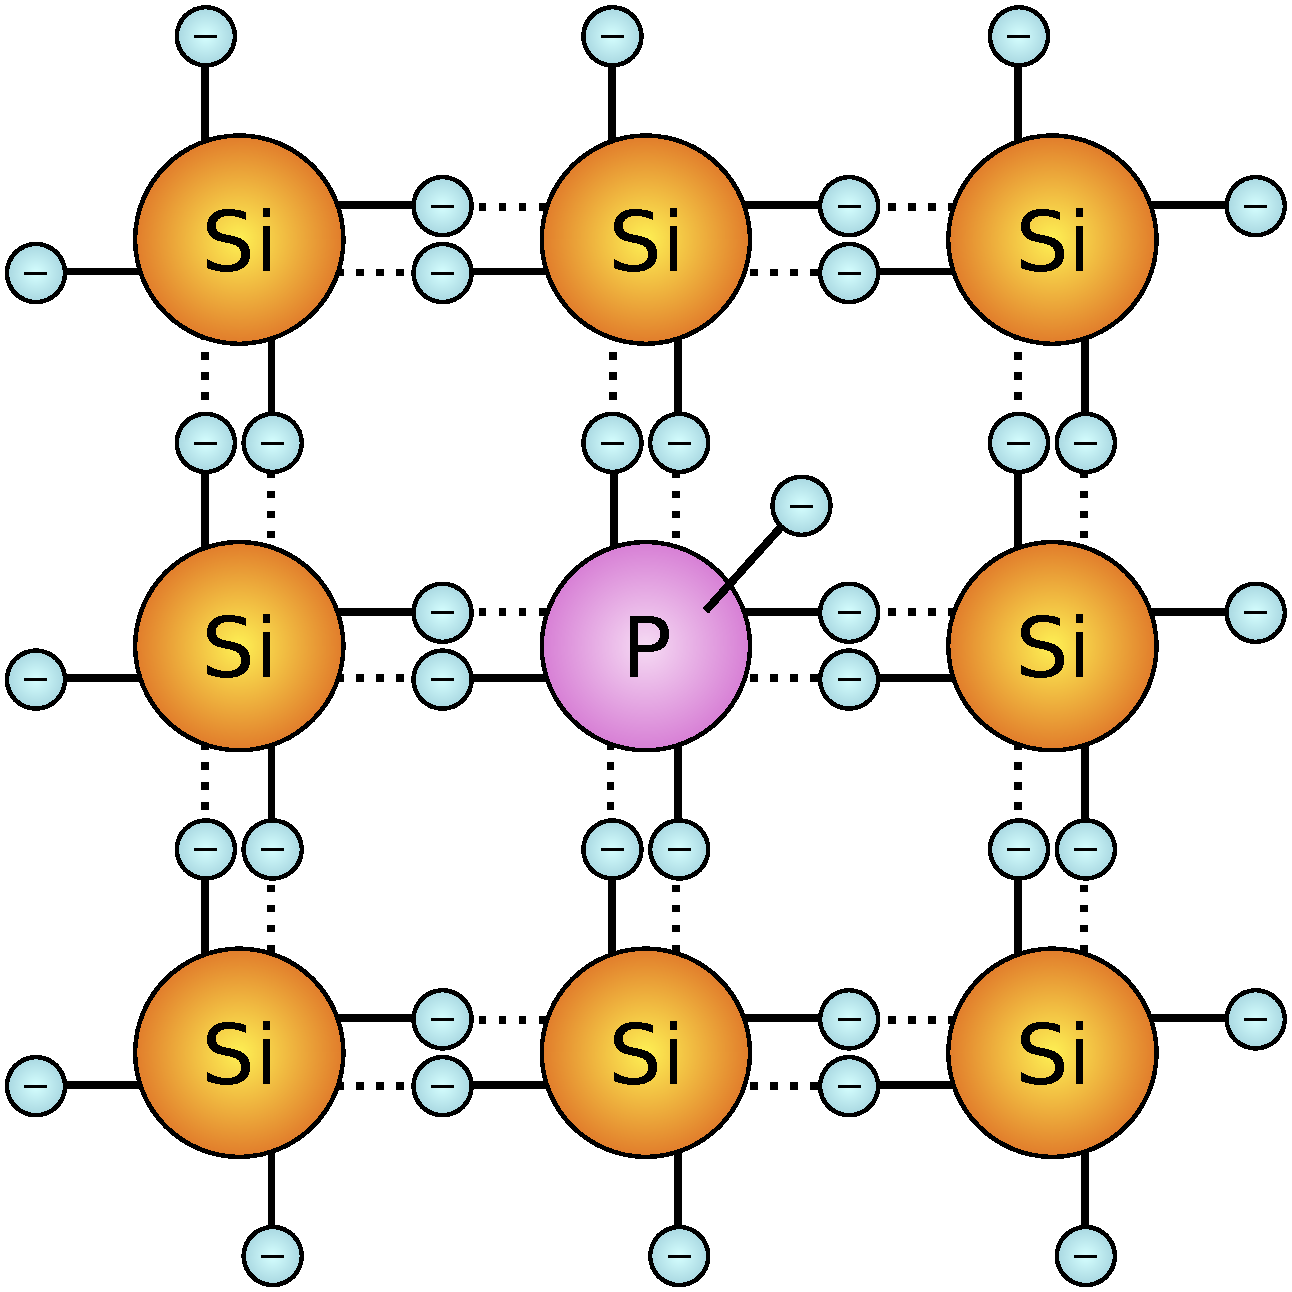
\includegraphics[width=.3\textwidth]{ndot.pdf}
  \label{img:ndot}
  \caption{n-Dotierung: Einbringen eines Fremdatoms zur Erzeugung eines Elektronenüberschusses}
\end{figure}

Als Beispiel der n-Dotierung wird in einen Silizium-Kristall (der über 4
Valenzelektronen verfügt) ein Phosphor-Atom eingebaut (das über 5
Valenzelektronen verfügt). Somit befindet sich im Kristall ein
Elektronenüberschuss (siehe Abbildung \ref{img:ndot}).

\begin{figure}[H]
  \centering
  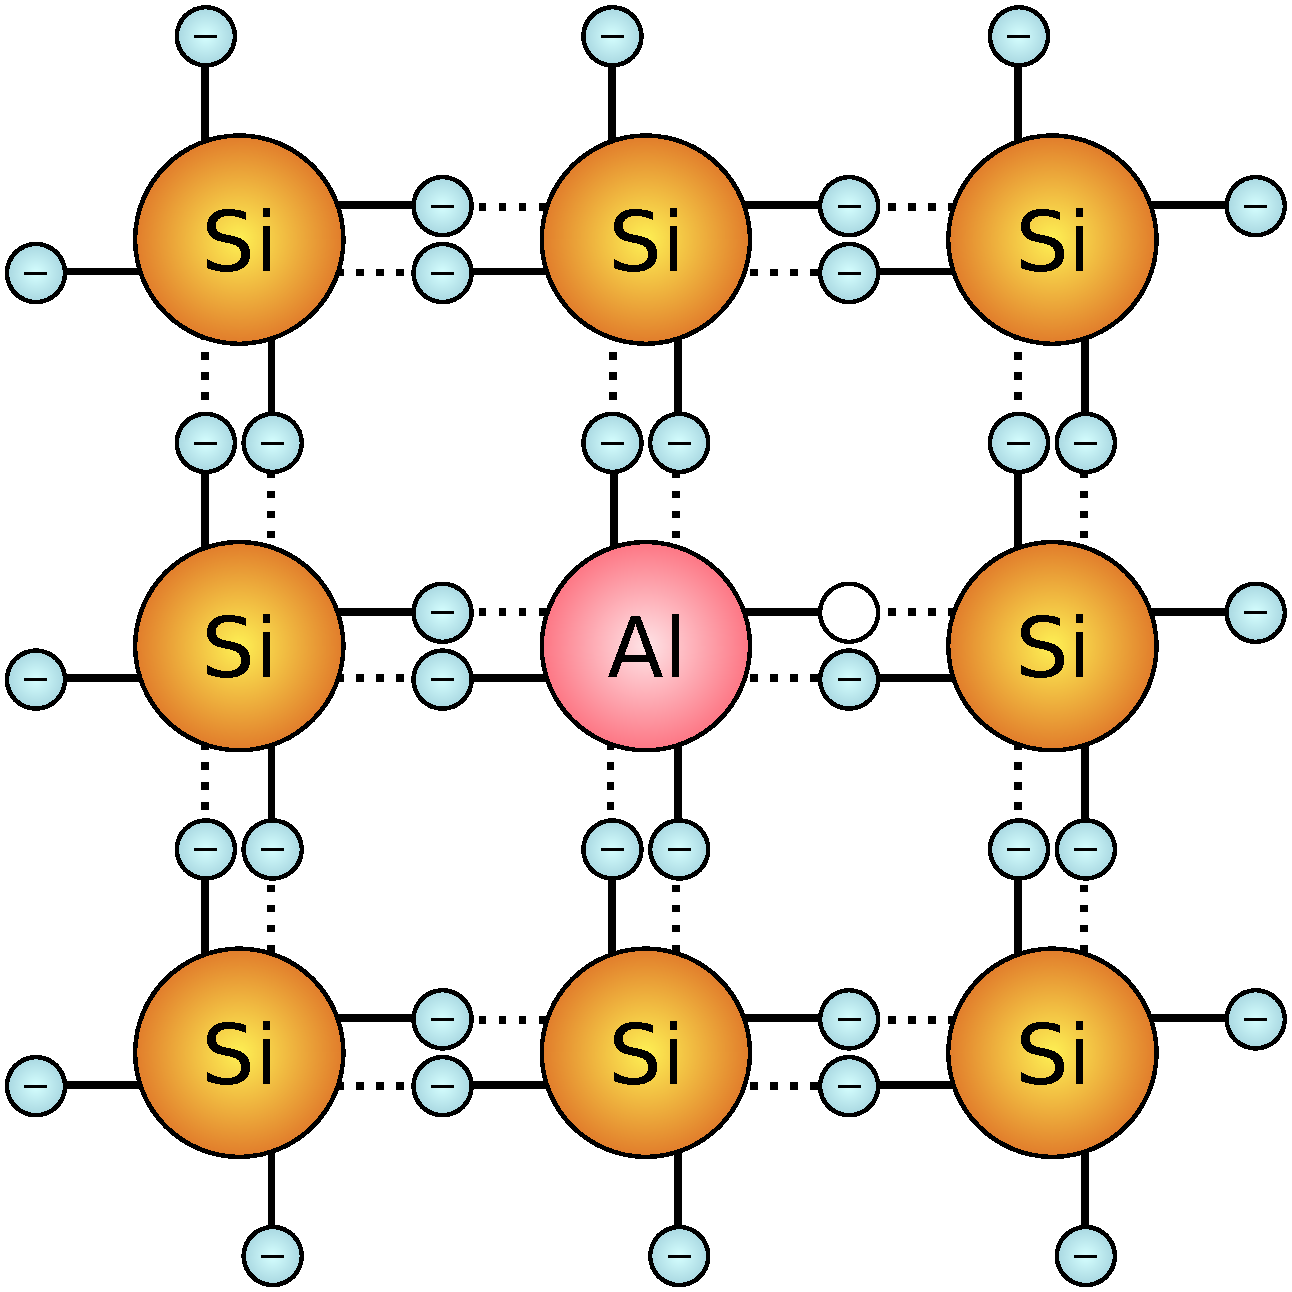
\includegraphics[width=.3\textwidth]{pdot.pdf}
  \label{img:pdot}
  \caption{p-Dotierung: Einbringen eines Fremdatoms zur Erzeugung einer Fehlstelle}
\end{figure}

Bei der p-Dotierung wird hingegen ein Aluminium-Atom (das über 3
Valenzelektronen) verfügt in den Kristall eingefügt. Es entsteht eine
Fehlstelle im Kristall (sog. Loch) (siehe Abbildung \ref{img:pdot}).

\begin{figure}[H]
  \centering
  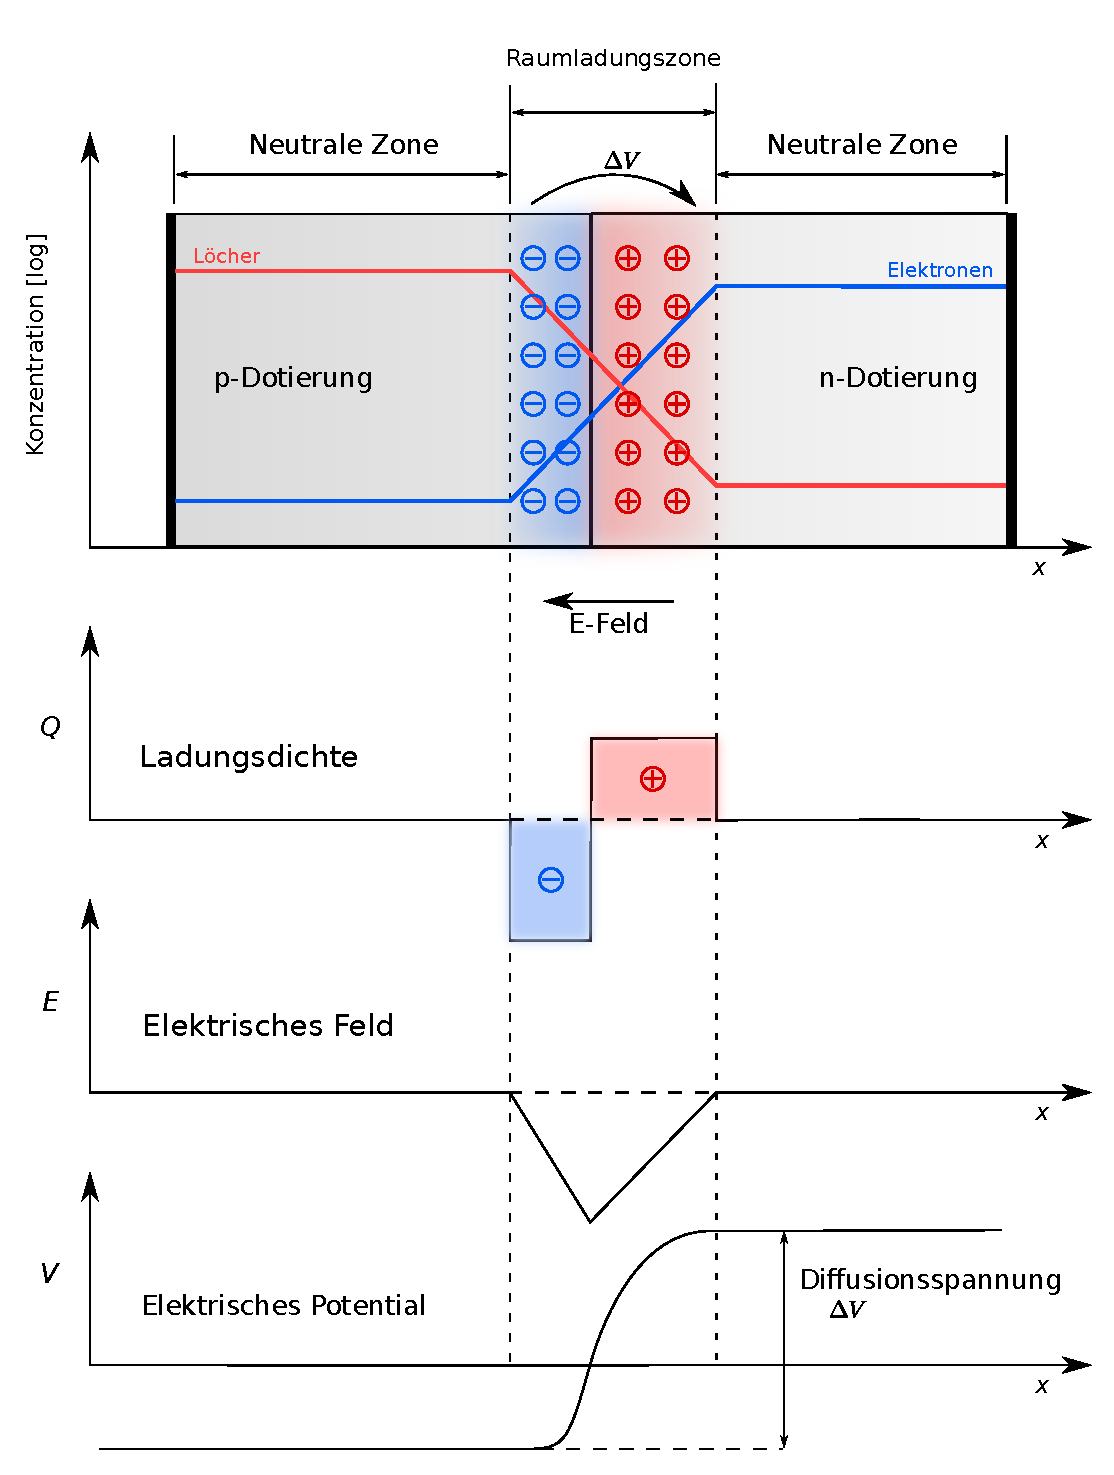
\includegraphics[width=.6\textwidth]{pnjunct.pdf}
  \label{img:pnjunct}
  \caption{p-n-Übergang}
\end{figure}

Eine Diode besteht nun aus einem p-n-Übergang. Das bedeutet, die beiden
dotierten Kristalle werden in direkten Kontakt miteinander gebracht. Dabei
rekombinieren die Elektronen mit den Löchern. Es entsteht ein elektrisches
Potential, das eine Sperrschicht bildet (siehe Abbildung
\ref{img:pnjunct}).

\subsubsection{Betrieb in Sperrrichtung}

Wird an die Diode eine Spannung angelegt (Minus am n-Kristall, Plus am
p-Kristall), kommen die Elektronen vom Minuspol und Rekombinieren mit den
Löchern. Dabei wird die Raumladungszone verbreitert und damit das zu
überwindende Potential höher. Es kann kein Strom fließen.

Wird irgendwann das Potential so groß, dass die Rekombinationszone gesättigt
wird und ist das Potential hoch genug, kommt es dennoch zum Durchtunneln
einzelner Elektronen (sog. Durchbruch). Diesen werden wir aber nicht messen.

\subsubsection{Betrieb in Durchlassrichtung}

Wird die Spannung anders herrum angelegt (Minus am p-Kristall, Plus am
n-Kristall) führt das dazu, dass die Elektronen die positive Ladung auf der
n-Seite kompensieren. Die Elektronen auf der p-Seite werden vom anliegenden
Potential zum Abfließen bewegt, somit verkleinert sich die Raumladungszone. Ist
die angelegte Spannung hoch genug (Durchlassspannung), ist die Raumladungszone
so klein, dass einzelne Elektronen durchtunneln können. Es beginnt ein Strom zu
fließen. Je hoher das Potential wird, desto kleiner wird die Raumladungszone
und desto mehr Elektronen fließen.

\subsubsection{Shockley-Gleichung}

Der Zusammenhang zwischen Strom- und Spannung an einer Diode wird durch die
Schockley-Gleichung angegeben. Diese lässt sich nur durch statistische
Betrachtungen an Halbleiterkristallen herleiten, weswegen ich auf die
Herleitung nicht genauer eingehen werde. Sie lautet:

\begin{equation}
  I_D = I_S \del{e^{U_D}{n U_T} - 1}
\end{equation}

Dabei gibt $I_D$ den Stromfluss durch die Diode bei einer angelegten Spannung
$U_D$ an. $n$ ist der materialabhängige Emissionskoeffizient ($n \in [1,2]$).
$U_T$ ist die Temperaturspannung $U_T = k_B T/q$ (mit $k_B$:
Boltzmann-Konstante, $T$: Temperatur, $q$: Elementarladung). Sie beträgt bei
Raumtemperatur etwa $25 \;\operatorname[mV]$.

\begin{figure}[H]
  \centering
  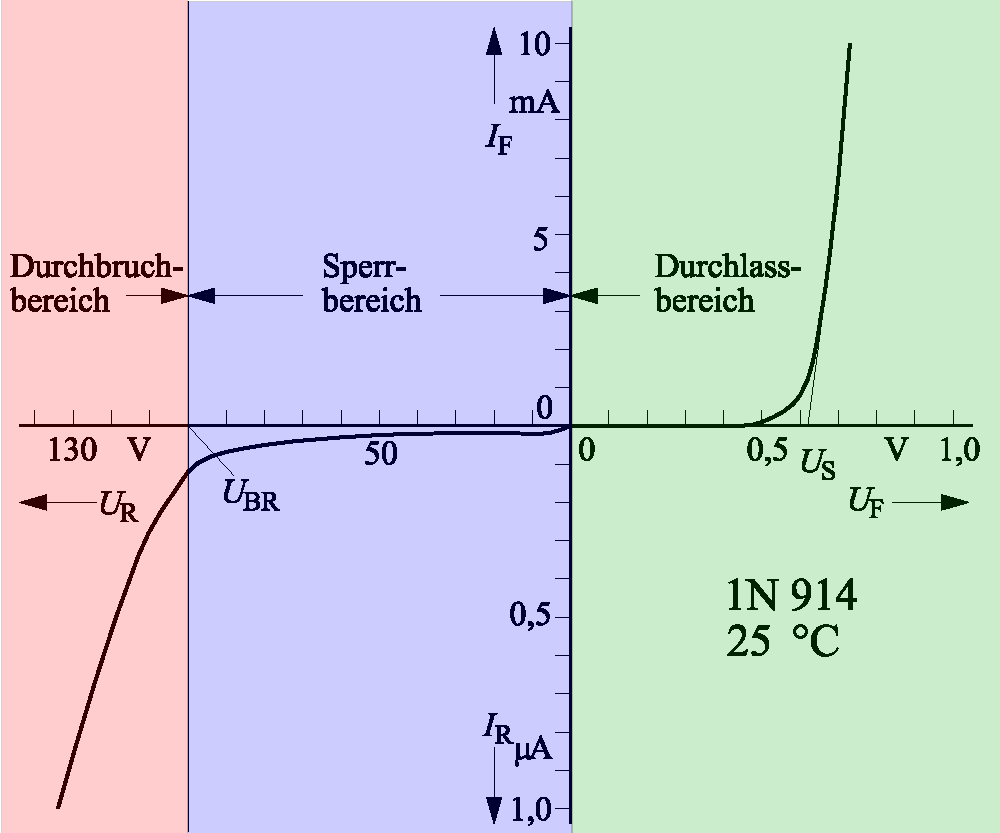
\includegraphics[width=.6\textwidth]{kennlinie.pdf}
  \label{img:kennlinie}
  \caption{Kennlinie einer Diode}
\end{figure}

Der Verlauf in Sperrrichtung folgt hingegen anderen Zusammenhängen, auf die
wir nicht weiter eingehen wollen, da wir diese nicht messen. Der Verlauf der
gesamten Kennlinie wird in Abbildung \ref{img:kennlinie} wiedergegeben.


\subsection{Elektrotechnische Betrachtungen}

\begin{figure}[H]
  \begin{center}
    \begin{circuitikz}
      \draw (0,0) to[Do] (2,0);
    \end{circuitikz}
    \caption{Schaltzeichen der Diode}
    \label{img:diode}
  \end{center}
\end{figure}

Das Schaltzeichen für die Diode ist in Abbilung \ref{img:diode} aufgeführt. Der
Pfeil zeigt dabei die Durchlassrichtung an, dabei gilt technische Stromrichtung
(also Stromfluss von Plus nach Minus).

\subsubsection{Einfacher Gleichrichter}

\begin{figure}[H]
  \begin{center}
\begin{tikzpicture}
    \draw (6,4) node[ocirc,label={right:+}] {};
    \draw (6,0) node[ocirc,label={right:--}] {};
    \draw (6,0)
      to[short] (0,0)
      to[sV] (0,4)
      to[Do] (6,4);

\end{tikzpicture}
    \caption{Einfacher Gleichrichter}
    \label{img:graetz}
  \end{center}
\end{figure}

\begin{figure}[H]
  \begin{center}
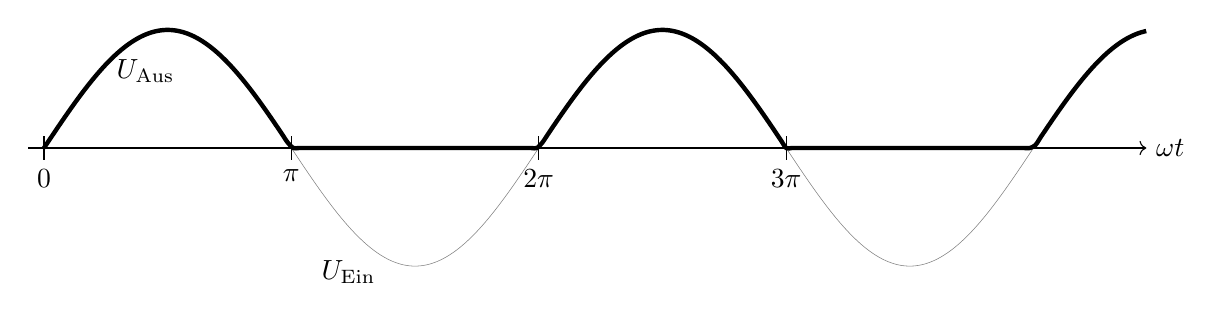
\begin{tikzpicture}
\begin{scope}[xscale=1,yscale=1.5]
    \draw[thin, ->] (-0.2, 0) -- (14,0) node[right] {$\omega t$};

    \foreach \x/\xtext in {0,{pi}/\pi,{2*pi}/{2\pi},{3*pi}/{3\pi}}
        \draw (\x,0.1) -- (\x,-0.1) node [below] {$\xtext$};


    % Vs
    \draw[domain=0:14, samples=200, help lines, smooth]
        plot (\x,{sin(\x r)});
    % U_0
    \draw[domain=0:14, samples=200, ultra thick, smooth]
      plot (\x,{max(sin(\x r), 0)});
    % U_Glatt
    %\draw[domain=0:14, thick, smooth]
    %  plot (\x,{1});
    \node[right] at (.8,.65) {$U_\text{Aus}$};
    %\node[right] at (1.7,1.25) {$U_\text{Glatt}$};
    \node[right] at ({pi+pi/12},-1.05) {$U_\text{Ein}$};
\end{scope}
\end{tikzpicture}
    \caption{Ein- und Ausgangsspannung des einfachen Gleichrichters}
    \label{img:simprectout}
  \end{center}
\end{figure}

Mithilfe der Diode lassen sich Wechselströme gleichrichten. Der naive Ansatz
ist dabei, eine einzelne Diode in Reihe zu einem Gleichstromverbraucher zu
schalten. Die Diode sperrt dann die negativen Halbwellen und lässt die
positiven durch. Dabei kann man jedoch nur jede zweite Halbwelle nutzen.

\subsubsection{Graetzschaltung}
\begin{figure}[H]
  \begin{center}
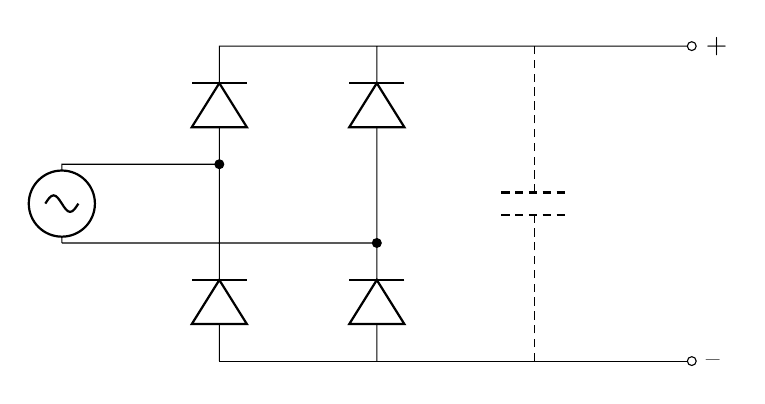
\begin{tikzpicture}
    \draw
    (2,0)
    % Diode leg 1
        to[Do] ++(0,1.5)
        -- ++(0,1)
        to[Do] ++(0,1.5) coordinate (leg2)
    % Diode leg 1
    (0,0)
        to[Do] ++(0,1.5)
        -- ++(0,1)
        to[Do] ++(0,1.5) coordinate (leg1)
    % Connections and load R
        -- ++(3,0)
        to[short] ++(3,0)
        %-- ++(0,-0.8)
        %to[R=$R_L$] ++(0,-2.4)
        %to[R] ++(0,-1.2)
        %to[L] ++(0,-1.2)
    % Back to (0,0)
        %|- (0,0)
    % AC source
    (-2,1.5) coordinate (Vnn)
        to[sV] ++(0,1) coordinate (Vpp)
        -- (leg1 |- Vpp) node [circ] {}
    (Vnn)
        -- (leg2 |- Vnn) node [circ] {}
    ;
    \draw (0,0) |- (6,0);
    \draw (6,4) node[ocirc,label={right:+}] {};
    \draw (6,0) node[ocirc,label={right:--}] {};
    \draw [densely dashed] (4,0) to[C] (4,4);
\end{tikzpicture}
    \caption{Graetzschaltung mit optionalem Glättungskondensator}
    \label{img:graetz}
  \end{center}
\end{figure}
\begin{figure}[H]
  \begin{center}
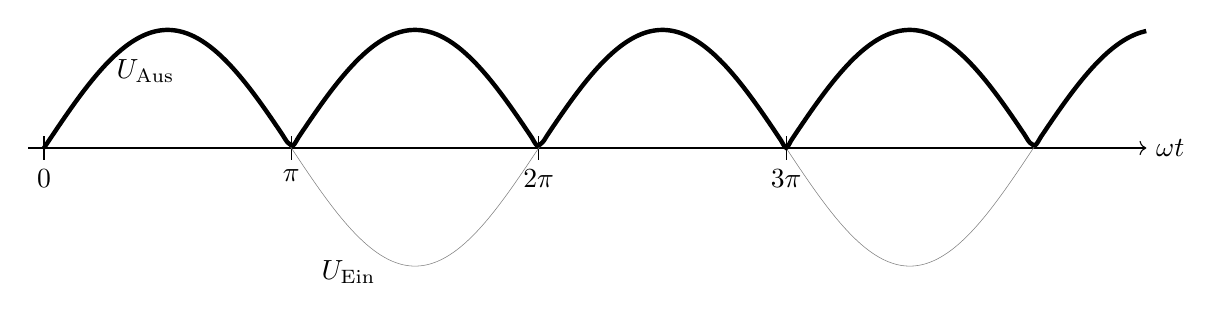
\begin{tikzpicture}
\begin{scope}[xscale=1,yscale=1.5]
    \draw[thin, ->] (-0.2, 0) -- (14,0) node[right] {$\omega t$};

    \foreach \x/\xtext in {0,{pi}/\pi,{2*pi}/{2\pi},{3*pi}/{3\pi}}
        \draw (\x,0.1) -- (\x,-0.1) node [below] {$\xtext$};


    % Vs
    \draw[domain=0:14, samples=200, help lines, smooth]
        plot (\x,{sin(\x r)});
    % U_0
    \draw[domain=0:14, samples=200, ultra thick, smooth]
      plot (\x,{abs(sin(\x r))});
    % U_Glatt
    %\draw[domain=0:14, thick, smooth]
    %  plot (\x,{1});
    \node[right] at (.8,.65) {$U_\text{Aus}$};
    %\node[right] at (1.7,1.25) {$U_\text{Glatt}$};
    \node[right] at ({pi+pi/12},-1.05) {$U_\text{Ein}$};
\end{scope}
\end{tikzpicture}
    \caption{Ein- und Ausgangsspannung einer Graetzschaltung}
    \label{img:graetzout}
  \end{center}
\end{figure}
Besser zur Gleichrichtung geeignet ist die Graetzschaltung. Dabei werden vier
Dioden genutzt (siehe Schaltung), um beide Halbwellen auszunutzen. Wir nehmen
dabei eine in erster Näherung lineare Kennlinie der Dioden an, um die
Betrachtung nicht zu komplex zu machen.


Wird noch ein Kondensator parallel zum Ausgang geschaltet, kann die Spannung
geglättet werden. Je nach Kennlinie der Dioden, angeschlossenem Verbraucher
usw. gibt es eine phasenverschobene Restwelligkeit. Die genaue Betrachtung ist
kompliziert und übersteigt die Aufgabenstellung. Da die intuitive Betrachtung
von nichtlinearen Wechselstromschaltkreisen zu falschen Ergebnissen führt,
sparen wir uns irgendwelche Mutmaßungen über das genaue Aussehen der
Ausgangsspannung in diesem Fall.



\end{document}

\newpage
\documentclass[a4paper,german,12pt,smallheadings]{scrartcl}
\usepackage[T1]{fontenc}
\usepackage[utf8]{inputenc}
\usepackage{babel}
\usepackage{geometry}
\usepackage[fleqn]{amsmath}
\usepackage{amssymb}
\usepackage{float}
\usepackage{enumerate}
\usepackage{commath} % http://tex.stackexchange.com/questions/14821/whats-the-proper-way-to-typeset-a-differential-operator
\usepackage{cancel}
\usepackage{pdfpages}

\usepackage[fleqn]{mathtools}
% Number only referenced equations
%\mathtoolsset{showonlyrefs}

%\usepackage{wrapfig}
\usepackage[thinspace,thinqspace,squaren,textstyle]{SIunits}
\usepackage{tikz}
\usepackage[europeanresistors]{circuitikz}

% New command for color underlining
\usepackage{xcolor}

\newsavebox\MBox
\newcommand\colul[2][red]{{\sbox\MBox{$#2$}%
  \rlap{\usebox\MBox}\color{#1}\rule[-1.2\dp\MBox]{\wd\MBox}{0.5pt}}}

\restylefloat{table}
\geometry{a4paper, top=15mm, left=20mm, right=10mm, bottom=20mm, headsep=10mm, footskip=12mm}
\linespread{1.5}
\setlength\parindent{0pt}
\DeclareMathOperator{\Tr}{Tr}
\DeclareMathOperator{\Var}{Var}
\begin{document}
\allowdisplaybreaks % Seitenumbrüche in Formeln erlauben
\begin{center}
\bfseries % Fettdruck einschalten
\sffamily % Serifenlose Schrift
\vspace{-40pt}
Physikalisches Grundpraktikum 2, Wintersemester 2014/2015

Markus Fenske \texttt{<iblue@zedat.fu-berlin.de>}

Transistor, Tutor: Andreas Maier
\vspace{-10pt}
\end{center}
\section{Einführung}
Ziel des Versuches ist die Aufnahme des Kennlinienfeldes eines
npn-Bipolartransistors  Außerdem soll eine Verstärkerstufe mit
Parallel-Gegenkopplung aufgebaut und die Verstärkung mit den theoretischen
Erwartungen verglichen werden.

\section{Theoretische Grundlagen}

\subsection{Transistor}

Der Transistor ist ein elektronisches Bauelement bei dem der Stromfluss auf
einer Strecke (Kollektor-Emitter) durch den Stromfluss auf der anderen Strecke
(Basis-Emmitter) gesteuert werden kann. Der Name leitet sich von
\textit{tran}sfer re\textit{sistor} ab, also einem steuerbaren Widerstand.

\subsubsection{Aufbau}

Anlog zur Diode handelt es sich um einen Aufbau aus dotierten Halbleitern
(Erklärung siehe dort). Im Unterschied zur Diode werden beim hier verwendeten
Transistor eine n-dotierte Schicht an eine p-dotierte Schicht und dann wieder
an eine n-dotierte Schicht gebracht. Es entstehen also zwei
Rekombinationszonen. Die n-dotierten Seiten heißen Kollektor und Emitter, die
p-Schicht in der Mitte Basis.

% FIXME: Grafik!
Wird der Transistor nun mit Kollektor und Emitter angeschlossen, leitet er in
keine Richtung, denn die Schaltung entspricht prinzipiell zwei gegeneinander
verschalteten Dioden. Die eine Sperrschicht wird zwar (bei genügend großer
Spannung) abgebaut, die andere jedoch vergrößert.

Betrachtet man den Betrieb in vorgesehener Richtung (Pluspol am Kollektor,
Minuspol am Emitter) ist nun also die Sperrschicht zwischen Basis und Emitter
abgebaut, die Sperrschicht zwischen Kollektor und Basis allerdings vergrößert.

Wir nun jedoch eine geringe Spannung zwischen Basis und Emitter angelegt,
beginnen Elektronen vom Emitter zur Basis zu fließen. Da die Sperrschicht
zwischen Basis und Kollektor jedoch klein ist und das Potential zwischen Basis
und Kollektor wesentlich größer ist, driften die meisten Elektronen direkt zum
Kollektor. Es fließt nun also ein Strom zwischen Kollektor und Emitter, der
Transistor leitet.

\subsubsection{Kennlinienfeld}

Die grundlegenden quantitativen Eigenschaften eines Transistors lassen sich im
Kennlinienfeld zusammenfassen. Es setzt die Ströme und Spannungen am Transistor
in Relation. Am Transistor lassen sich drei Spannungen messen. Die Spannung
zwischen Kollektor und Emitter ($U_{CE}$), die Spannung zwischen Basis und
Emitter ($U_{BE}$) und die Spannung zwischen Kollektor und Basis ($U_{CB}$). Da
das elektrische Feld konservativ ist, gilt

\begin{equation}
  U_{CE} = U_{CB} + U_{BE}
\end{equation}

Außerdem lassen sich die Ströme an Basis, Emitter und Kollektor messen.
Aufgrund der Ladungserhaltung gilt dann

\begin{equation}
  I_C + I_B + I_E = 0
\end{equation}

Somit bleiben vier freie Parameter, die durch das Kennlinienfeld jeweils in
Relation gesetzt werden, um das Verhalten des Transistors zu beschreiben.

\begin{figure}[H]
  \centering
  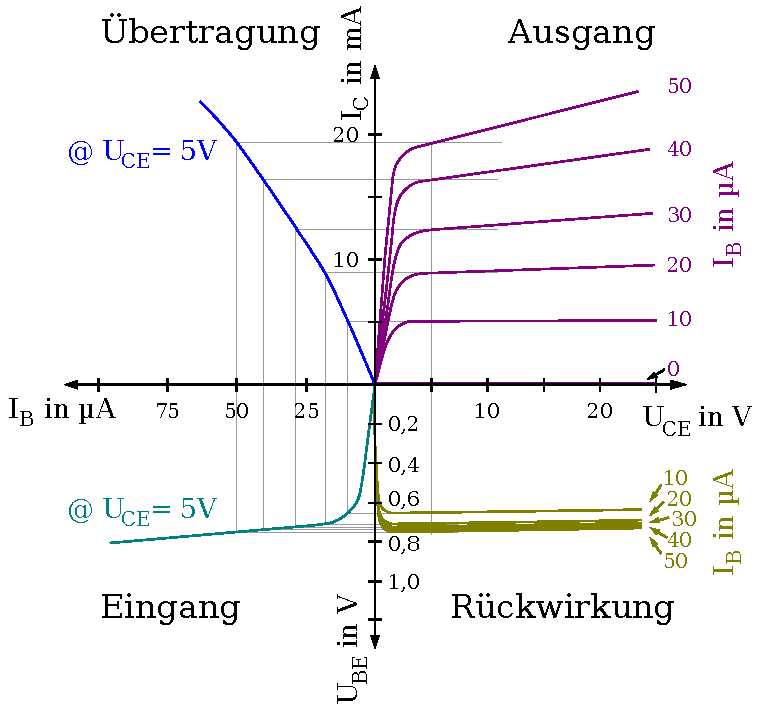
\includegraphics[width=.6\textwidth]{kennlinienfeld.pdf}
  \label{img:kennlinie}
  \caption{Kennlinienfeld eines Transistors}
\end{figure}

Im ersten Quadranten lässt sich der \textit{Ausgangswiderstand} ablesen. Er
gibt das Verhältnis Emitter-Kollektor-Spannung $U_{CE}$ und dem Kollektorstrom
$I_C$ an.

Im zweiten Quadranten wird das Stromsteuer-, Übertragungs- oder auch
Stromverstärkungskennlinienfeld dargestellt. Es setzt Basis- und Kollektorstrom
in Relation und bestimmt damit den Verstärkungsfaktor.

Im dritten Quadranten lässt sich der Eingangswiderstand ablesen. Er gibt das
Verhältnis zwischen Basis-Emitter-Spannung $U_{BE}$ und Basisstrom $I_B$ an.

Im vierten Quadranten ist die Spannungsrückwirkung aufgetragen, sie gibt das
Verhältnis der beiden obigen Spannungen an.

Oft wird ins Kennlinienfeld auch die \textit{Leistungshyperbel} aufgetragen.
Der Ausgangswiderstand des Transistors führt nämlich zu einer Verlustleistung
und damit zur Erwärmung des Transistors. Um eine Überhitzung zu vermeiden, darf
die Leistung eine Grenze $P = UI$ nicht überschreiten. Trägt man $I$ in
Abhängigkeit von $U$ bei konstanten $P$ auf, ergibt sich somit eine Hyperbel.

\begin{equation}
  U(I) = \frac{P}{I}
\end{equation}

Der Aufbau zur Aufnahme des Kennlinienfeldes ist in der folgenden Abbildung
dargestellt. Es kann der Basisstrom und die Emitter-Kollektor-Spannung variiert
werden, um die jeweiligen Parameter aufzunehmen.

\begin{figure}[H]
  \begin{center}
    \begin{circuitikz}
      \draw (0,0)
      to[battery1=$1{,}5V$] (0,2)
      to[ammeter,l=$I_B$] (2,2)
      to[R=$2{,}2\;\text{k}\Omega$] (4,2)
      to[vR=$22\;\text{k}\Omega\;\text{(log)}$] (6,2)
      to[voltmeter,l=$U_{EB}$] (6,0)
      to[short] (0,0);
      \draw (8,2) node[npn] (npn) {}
      (npn.base) node[anchor=south] {B}
      (npn.collector) node[anchor=west] {C}
      (npn.emitter) node[anchor=west] {E};
      \draw (6,2) |- (npn.base);
      \draw (6,0) -| (npn.emitter);
      \draw (6,0)
      to[short] (12,0)
      to[V,v=$U_0$] (12,6)
      to[short] (10,6)
      to[ammeter,l=$I_C$] (10,3.5)
      -| (npn.collector);
      \draw (10,4)
      to[voltmeter,l=$U_{EC}$] (10,0);
    \end{circuitikz}
    \caption{Aufbau zur Messung des Kennlinienfeldes}
  \end{center}
\end{figure}

\subsubsection{Verstärkerschaltung}

Möchte man eine Wechselspannung verstärken, müssen einige Maßnahmen zur
Signalanpassung getroffen werden. Da der Transistor nur positive
Basis-Emitter-Ströme verstärkt, muss das Potential des Signals angehoben
werden. Wird der erreichte Punkt im Kennlinienfeld dargestellt, spricht man von
Arbeitspunkt.

Um nur Wechselspannungen zu verstärken, wird das Signal jeweils durch
einen Koppelkondensator an Ein- und Ausgang gefiltert.

Da Halbleiter stark temperaturabhängig sind, möchte man den Arbeitspunkt
stabilisieren um ein gleichmäßiges Verhalten bei unterschiedlichen Temperaturen
zu erreichen. Dazu nutzt man die \textit{Gegenkopplung}. Dabei wird ein Teil
des Ausgangsstroms über einen Widerstand zurückgeführt um den Arbeitspunkt
entsprechend zu verschieben. Ist der Emitterstrom bei höherer Temperatur
größer, senkt dies den Arbeitspunkt auf einen geringeren Wert (siehe Schaltung).

\begin{figure}[H]
  \begin{center}
    \begin{circuitikz}
      \draw (4,2) node[npn] (npn) {}
      (npn.base) node[anchor=south] {B}
      (npn.collector) node[anchor=west] {C}
      (npn.emitter) node[anchor=west] {E};
      \draw (0,2)
      to[C=$C_k$] (1.5,2) % Bisschen Platz machen, sonst label kaputt.
      to[short]   (2,2)
      to[short] (npn.base);
      \draw (0,0) -| (npn.emitter) |- (6,0);
      \draw (2,2)
      to[R=$R_V$] (2,4)
      to[short] (4,4) |- (npn.collector);
      \draw (4,4)
      to[C=$C_k$] (6,4);
      \draw (4,4)
      to[R=$R_A$] (4,6)
      to[short] (6,6);
      \draw (6,6) node[anchor=west] {12V};
      \draw (6,4) node[anchor=west] {Aus};
      \draw (6,0) node[anchor=west] {0V};
      \draw (0,2) node[anchor=east] {Ein};
      \draw (0,0) node[anchor=east] {0V};
    \end{circuitikz}
    \caption{Verstärkerschaltung mit Gegenkopplung}
  \end{center}
\end{figure}

\section{Aufgaben}
\begin{enumerate}
  \item Aufnahme und Konstruktion des statischen Kennlinienfeldes eines
    npn-Transistors bei einer Versorgungsspannung von 12V. Bestimmung der
    Stromverstärkung für den statischen Fall.
  \item Aufbau einer Verstärkerschaltung mit Parallelgegenkopplung und
    Verstärkung einer Eingangswechselspannung.
\end{enumerate}


\end{document}

\newpage
\documentclass[a4paper,german,12pt,smallheadings]{scrartcl}
\usepackage[T1]{fontenc}
\usepackage[utf8]{inputenc}
\usepackage{babel}
\usepackage{geometry}
\usepackage[fleqn]{amsmath}
\usepackage{amssymb}
\usepackage{float}
\usepackage{enumerate}
\usepackage{commath} % http://tex.stackexchange.com/questions/14821/whats-the-proper-way-to-typeset-a-differential-operator
\usepackage{cancel}
\usepackage{pdfpages}

\usepackage[fleqn]{mathtools}
% Number only referenced equations
%\mathtoolsset{showonlyrefs}

%\usepackage{wrapfig}
%\usepackage[thinspace,thinqspace,squaren,textstyle]{SIunits}
\usepackage{tikz}
\usepackage[europeanresistors]{circuitikz}

\usepackage{siunitx}
\sisetup{separate-uncertainty=true,locale=DE}

% New command for color underlining
\usepackage{xcolor}

\newsavebox\MBox
\newcommand\colul[2][red]{{\sbox\MBox{$#2$}%
  \rlap{\usebox\MBox}\color{#1}\rule[-1.2\dp\MBox]{\wd\MBox}{0.5pt}}}

\restylefloat{table}
\geometry{a4paper, top=15mm, left=20mm, right=10mm, bottom=20mm, headsep=10mm, footskip=12mm}
\linespread{1.5}
\setlength\parindent{0pt}
\DeclareMathOperator{\Tr}{Tr}
\DeclareMathOperator{\Var}{Var}
\begin{document}
\allowdisplaybreaks % Seitenumbrüche in Formeln erlauben
\begin{center}
\bfseries % Fettdruck einschalten
\sffamily % Serifenlose Schrift
\vspace{-40pt}
Physikalisches Grundpraktikum 2, Wintersemester 2014/2015

Markus Fenske \texttt{<iblue@zedat.fu-berlin.de>}

E-Block, Tutor: Andreas Maier
\vspace{-10pt}
\end{center}
\section{Auswertung}

\subsection{Aufgaben}
\begin{enumerate}
  \item \textbf{Lade-/Entladekurve Kondensator}
    \begin{enumerate}
      \item  Bestimmung der Zeitkonstanten und Kapazität des Kondensators und
        Vergleich mit den berechneten Werten
      \item Diskussion des Einflusses der Frequenz der Rechteckspannung auf die
        Lade-/Entladekurven
    \end{enumerate}
  \item \textbf{Diode}
    \begin{enumerate}
      \item Bestimmung der Schwellenspannung sowie des (differentiellen)
        Wiederstandes im Durchlassbereich
      \item Zusatzaufgabe: Bestimmung des Idealitätsfaktors $n$ bei einer
        Temperatur von $20\,^\circ C$.
    \end{enumerate}
  \item \textbf{Transistor}
    \begin{enumerate}
      \item Bestimmung des differentiellen Ausgangswiderstandes im
        Durchlassbereich für Basisströme von 30, 60, 90 und 120 $\mu$A
      \item Bestimmen des Gleichstromverstärkungsfaktors
      \item Bestimmung des Arbeits- und Vorwiderstands aus dem aufgenommenen
        Kannlinienfeld für einer Verstärkerschaltung bei $U_\text{CE} = 6
        \text{V}$.
    \end{enumerate}
\end{enumerate}

\subsection{Lade-/Entladekurve des Kondensators}

Umstellen und Logarithmieren der Auf- und Entladekurve führt zu den
linearisierten Messgleichungen

\begin{equation}
  \ln \frac{U_C}{U_0} = -\frac{t}{RC} \qquad \text{(Entladekurve)}
\end{equation}

und

\begin{equation}
  \ln \del{1 - \frac{U_C}{U_0}} = -\frac{t}{RC} \qquad \text{(Aufladekurve)}
\end{equation}

eine entsprechende logarithmische Auftragung und linearer Fit (siehe Plot)
liefert direkt die Zeitkonstanten (Aufladung und Entladung)

\begin{equation}
  \tau = \num{1.65+-0.11} \; \text{ms}
\end{equation}

und

\begin{equation}
  \tau = \num{1.722+-0.065} \; \text{ms}
\end{equation}

Die beiden Werte sind verträglich. Das Endergebnis der Zeitkonstante ergibt
sich als Mittelung $(a+b)/2$ und dem Fehler (per Gauß) $\Delta = \sqrt{\Delta
a^2 + \Delta b^2}/2$.

\begin{equation}
  \tau = \num{1.69\pm0.07} \; \text{ms}
\end{equation}

Der theoretische Wert der Zeitkonstante ist $\tau =
\num{18.0+-0.9}\,\text{k}\Omega \cdot 0{,}1\,\mathrm{\mu} \text{F} =
\num{1.8+-0.9} \, \text{ms}$. Der Widerstand wurde nicht gemessen, eine
Minimalabschätzung des Fehlers ergibt sich aus ergibt sich aus der bei
Kohleschichtwiderständen üblichen Fertigungstoleranz von 5 \%. Der Fehler des
Kondensators ist unbekannt, wird daher aufgrund der Minimalabschätzung
vernachlässigt.

Der experimentell ermittelte Wert der Zeitkonstante ist mit dem theoretischen
Wert identisch.

Zur Bestimmung der Frequenz des Kondensators wird einfach durch den Widerstand
geteilt. Es gilt

\begin{equation}
  C = \frac{\tau}{R}
\end{equation}

mit dem Fehler
\begin{equation}
  \Delta C = \sqrt{
    \del{\frac{\partial C}{\partial R} \Delta R}^2 +
    \del{\frac{\partial C}{\partial \tau} \Delta \tau}^2
  }
  = \sqrt{
    \frac{\tau^2 \Delta R^2}{R^4} + \frac{\Delta \tau^2}{R^2}
  }
\end{equation}

Somit ist die Kapazität (als Endergebnis):
\begin{equation}
  C = \num{0.094+-0.007} \;\mu\text{F}
\end{equation}

Der Wert ist mit dem angegebenen Wert von $C = 0{,}01 \; \mu\text{F}$
identisch. Er zeigt außerdem, dass die Toleranzabschätzung von 5 \% korrekt
war.

Die Frequenz der Rechteckspannung hat einen Einfluss auf die
Lade/Entladekurve. Bei der verwendeten Frequenz von 50 Hz scheinen noch keine
Auswirkungen aufzutreten, wie die Übereinstimmung der experimentellen Resultate
mit den theoretischen Werten zeigen, jedoch kommen folgende Möglichkeiten in
Frage.

Abschwächung der End/Anfangsspannung: Ist die Periode geringer, wird der
Kondensator nicht lange genug geladen um sich der Endspannung anzunähern. Man
kann dann Spannung beim Phasenwechsel nicht mehr als näherungsweise $U_0$
betrachten. Dies würde zu einem systematischen Fehler führen, sofern man nicht
Endspannung und $U_0$ am Oszilloskop vergleicht. Da beiden Spannungen
gleichzeitig betrachtet werden müssen, nimmt dann jedoch die Spannung am
Kondensator einen geringeren Platz auf dem Oszilloskop ein, was die
Ablesegenauigkeit verringert.

Hochfrequenzeffekte: Bei höheren Frequenzen treten möglicherweise
Hochfrequenzeffekte auf. Zu berüchsichtigen wäre die Induktivität der
Verbindungskabel, die Repolarisationszeit des Dielektrikums des Kondensators
und eventuelle Phasenverschiebungen (lässt sich theoretisch eventuell durch
Entwicklung des Rechtecksignals in eine Fourierreihe und dann Behandlung der
einzelnen Frequenzen im Rahmen der komplexen Wechselstromrechnung), sowie
Reflektionen an Kabeln etc. Da diese Themen den Umfang des Grundpraktikums
übersteigen, werde ich darauf nicht weiter eingehen.

\subsection{Diode}

Die Schwellenspannung ergibt sich durch Verlängerung des scheinbar geradlinigen
Teils der Kennlinie. Da die Kennlinie der Shockley-Gleichung entspricht,
existiert die Schwellspannung mathematisch überhaupt nicht. Die Steigung geht
gegen 1 (ersichtlich durch Grenzwertbildung der Ableitung der
Shockley-Gleichung). Da die Gleichung selber $U$-Werte von unendlich erreicht,
ergibt die senkrechte Projektion auf die x-Achse auch einen unendlichen Wert.
Der differentielle Widerstand wird ebenfalls unendlich. Um dennoch eine
Schwellenspannung und einen entsprechenden Fehler zu berechnen, führe ich eine
lineare Regression auf den letzten 5 Messwerten durch (siehe Plot). Dazu nutze
ich die Werte der spannungrichtigen Messung.

Durch Ablesen der Projektion auf die x-Achse ergibt sich eine Schwellenspannung
von

\begin{equation}
  U_S = \num{0.72+-0.03} \text{V}
\end{equation}

Eine andere Definition der Schwellenspannung ist die Spannung, bei der der
Strom 1 mA erreicht. Auch dies lässt sich ablesen und führt auf eine
Schwellenspannung von
\begin{equation}
  U_S = \num{0.60\pm0.01} \text{V}
\end{equation}

Die beiden Werte sind nicht verträglich. Dies liegt daran, dass die
Schwellenspannung messabhängig definiert ist.

Die Berechnung eines differentiellen Widerstands ist ebenso messabhängig. Er
ergibt sich aus der Steigung der Regressionsgerade. Diese ist nach Rundung

\begin{equation}
  1/R_D = \num{990\pm590} / k \Omega
\end{equation}

Den Widerstand erhält man durch Bildung des Inversen. Der Fehler ist dann
$\Delta R_D = \frac{\Delta(1/R_D)}{R_D^2}$.

Das Endergebnis lautet
\begin{equation}
  R_D = \num{1.0+-0.6} \,\Omega
\end{equation}

Die geringe Genauigkeit liegt in der messabhängigen Definition der
Schwellenspannung begründet.

Zusatzaufgabe: Nicht bearbeitet.




\end{document}

\newpage
\invisiblesection{Plots}
\subimport{messdaten/2/}{render-plot.tex}
\newpage
\subimport{messdaten/3/}{render-plot.tex}
\newpage
\subimport{messdaten/4/}{render-plot.tex}
\newpage
\invisiblesection{Messprotokolle und im Praktikum angefertigte Plots}


\end{document}
